\chapter[Sapphire AR coating]{Sapphire anti-reflection coating}
\label{ch:sapphire_ar_coating}

The final component of the cryogenic half-wave plate (CHWP) system is the sapphire's anti-reflection (AR) coating. Sapphire has an crystal-axis-averaged refractive index of $n_{\mathrm{sapphire}} \approx 3.2$, and therefore the Fresnel reflection coefficient at normal incidence\footnote{Reflectivity increases at non-normal incidence, and therefore this bare-sapphire reflectivity represents a lower limit.} is
\begin{equation}
    R = \frac{\left( n_{\mathrm{sapphire, avg}} - n_{\mathrm{vacuum}} \right)^{2}}{\left( n_{\mathrm{sapphire, avg}} + n_{\mathrm{vacuum}} \right)^{2}} \approx 0.3
    \label{eq:sapphire_reflection_coefficient}
\end{equation}
where the refractive index of vacuum $n_{\mathrm{vacuum}} = 1$. This level of reflection at any refractive optic in the experiment has several problematic ramifications, including decreased optical throughput, beam distortions, and multiple reflections within the cryostat the generate \important{ghosting}, or the formation of ``ghost'' images. The purpose of an AR coating is to reduce \important{reflectivity}---or the fraction of incident power reflected back towards the source---in order to limit these undesired effects, and therefore AR coatings are among the most active and important research areas in CMB instrumentation today. 

The quality of the CHWP AR coating is critical to its effectiveness. In addition to reducing its axis-averaged reflectivity, the AR coating suppresses differential transmission between the ordinary axis with $n_{\mathrm{o}} \approx 3.08$ and extraordinary axis with $n_{\mathrm{e}} \approx 3.35$, which in turn suppresses the amplitude of the $2f_{\mathrm{HWP}}$ HWP synchronous signal (HWPSS) (see Section~\ref{sec:hwp_synchronous_signals}). Without any AR coating, this differential reflectivity is $\Delta R = R_{\mathrm{e}} - R_{\mathrm{o}} \approx 3$\%, which for 10~K of atmospheric loading (see Figure~\ref{fig:so_bands_atacama}) corresponds to a $\approx$~300~mK signal. This HWPSS will have a harmonic component at $4 f_{\mathrm{HWP}}$ for light at non-normal incidence~\cite{salatino_studies_2018}, and therefore an important role of the sapphire AR coating is to suppress it. In addition to minimizing reflections, the CHWP AR coating must be highly uniform, as nonuniformities in the Pancharatnam stack induce HWPSSs in the detector data that can be difficult to remove during analysis. For these reasons, developing high-quality AR coatings is an emphasis of the CHWP development.

There are many methods used to AR coat mm-wave optics, and with the recent rise of polarization modulators, several of these methods are beginning to be applied to sapphire. In this chapter, we cover the coatings that have been developed specifically for the Simons Array (SA) CHWP. For a discussion of the CHWP sapphire---which is identical to that of the PB-2a warm HWP (WHWP)---see Section~\ref{sec:pb2a_whwp_sapphire}, and for a related discussion of the WHWP AR coating development, see Section~\ref{sec:pb2a_whwp_ar_coating}.

%%%%%%%%%%%%%%%%%%%%%%%%%%%%%%%%
%%%%%%%%%%%%%%%%%%%%%%%%%%%%%%%%
%%%%%%%%%%%%%%%%%%%%%%%%%%%%%%%%

\section{AR coating design}
\label{sec:sapphire_ar_coating_design}

An AR coating suppresses reflectivity by gradually transforming the refractive index from that of air/vacuum $n_{\mathrm{vacuum}} = 1$ to that of the refractive optic. The more gradual the transformation, the less light is reflected, and therefore in the absence of practical considerations, more AR layers generally correspond to lower reflectivity.\footnote{The statement that more AR layers lead to lower reflectivity is not \textit{always} true, as the wavelength, layer thicknesses, and indexes of the AR coating matter, but assuming the coating is designed to decrease reflections over a given bandwidth, more layers indeed perform better.} In addition, reflection can be suppressed further by tuning each layer's thickness 
\begin{equation}
    d_{\lambda / 4} = \lambda_{0} / (4 n)
    \label{eq:lambda_over_four_thickness}
\end{equation}
to maximize destructive interference between forward- and backward-traveling light, where $\lambda_{0}$ is the wavelength of the incident light in a vacuum and where $n$ is the AR layer's refractive index. This construction is called a \important{quarter-wave} coating and if all layers are $d_{\lambda / 4}$, it has zero reflection for incident light of wavelength $\lambda_{0}$.

\begin{figure}[!t]
    \centering
    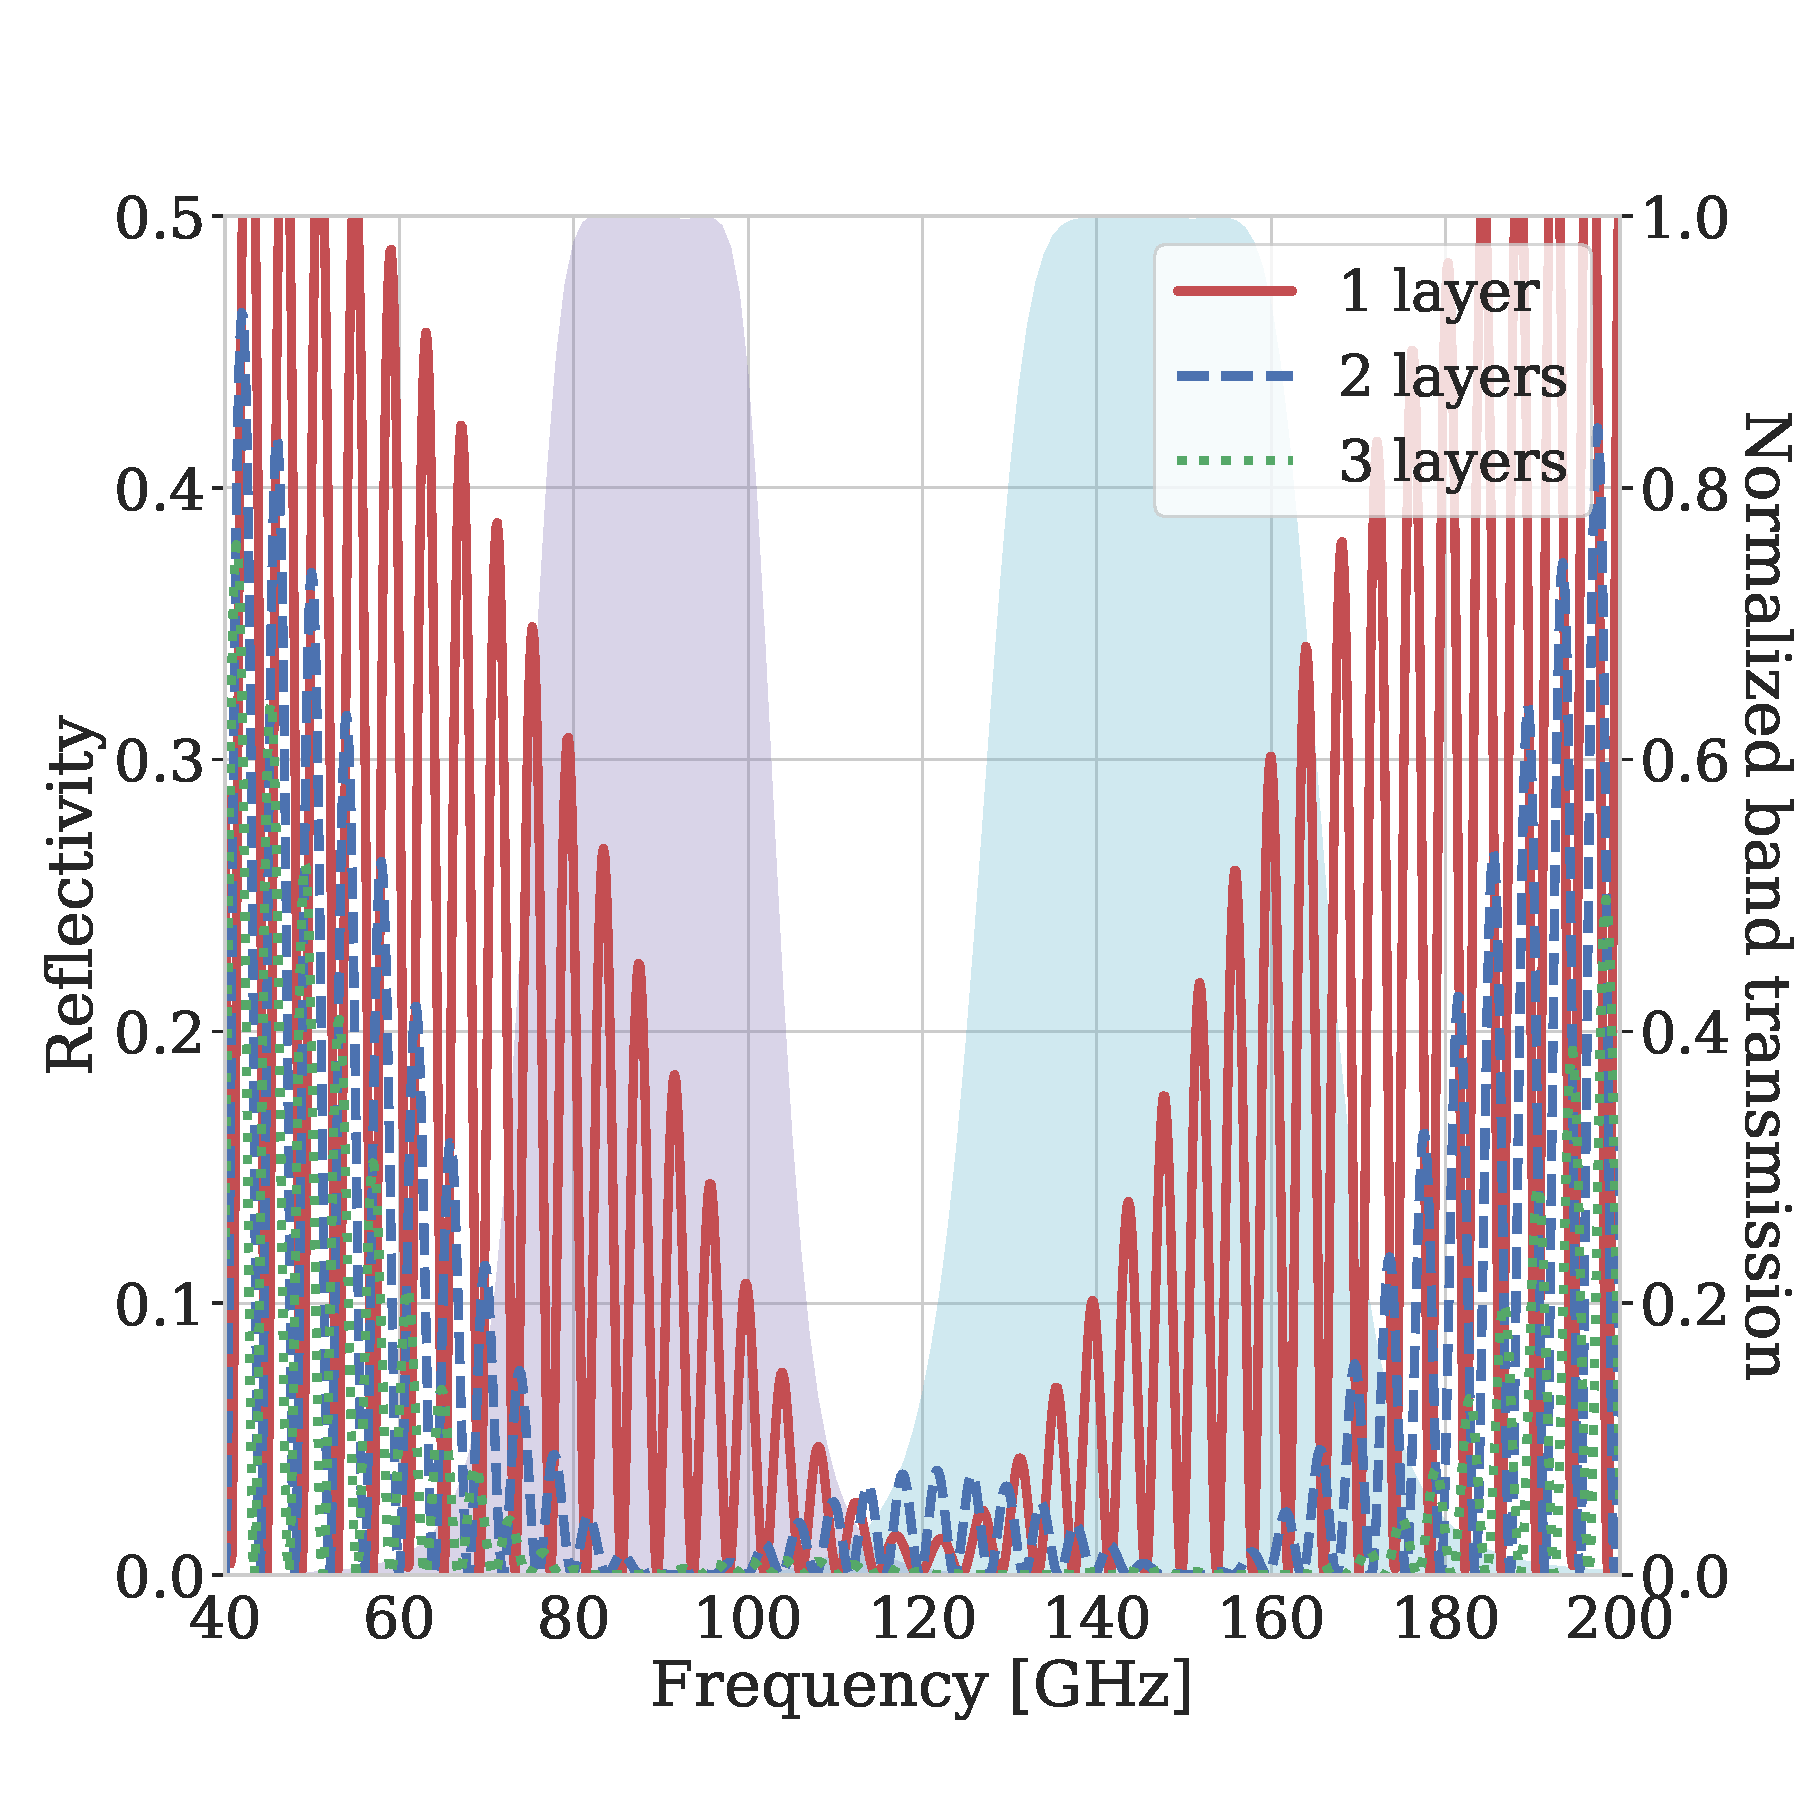
\includegraphics[width=0.5\linewidth, trim=1cm 1cm 1cm 2cm, clip]{ARCoating/Figures/one_two_three_layer_ar_optimize.pdf}
    \begin{tabu}{| c | c | c | c | c |}
        \hline
        Layers & $n_{\mathrm{AR}}$ & $d_{\mathrm{AR}}$ [$\mathrm{\mu m}$] & $R_{90}$ [\%] & $R_{150}$ [\%] \\
        \hline
        \hline
        1 & (1.70) & (367) & 11.6 & 9.7 \\
        \hline
        2 & (1.41, 2.29) & (437, 269) & 1.1 & 1.1 \\
        \hline
        3 & (1.21, 1.80, 2.67) & (494, 339, 223) & 0.3 & 0.1 \\
        \hline
    \end{tabu}
    \caption[Comparison of one-, two-, and three-layer AR coatings for the PB-2b CHWP.]{Comparison of a one-, two-, and three-layer AR coatings optimized to maximize the average transmissivity across the 90 (magenta) and 150~GHz (cyan) detector bands. The sapphire substrate is assumed to have a thickness of 11.25~mm and an axis averaged refractive index of $n_{\mathrm{sapphire}} = 3.23$. The optimal indexes, thicknesses, and resulting reflectivity in each band is shown in the table. The largest transmissivity improvement comes between the one- and two-layer coatings.}
    \label{fig:one_two_three_layer_ar_coating_optimization}
\end{figure}

From the perspective of PB-2b, which has a fixed observation bandwidth, adding more layers to the AR coating effectively adds more degrees of freedom over which the coating can be optimized, which in turn can be used to better suppress reflectivity. Figure~\ref{fig:one_two_three_layer_ar_coating_optimization} shows the a fully\footnote{``Fully'' means that all layer thicknesses and indexes are allowed to float during the optimization.} optimized~\cite{Hou1974MethodFilters} one-, two-, and three-layer coating and their resulting reflectivities integrated across the PB-2b 90 and 150~GHz bands. A single-layer coating has insufficient bandwidth to achieve reasonable reflectivity in both bands, and therefore, despite the strong heritage of one-layer coatings in single-color CMB experiments, the PB-2b CHWP must employ a multi-layer coating. A two-layer coating does substantially better, achieving 1.1\% reflection in each band, and the three-layer coating does even better, achieving (0.3, 0.1)\% reflection at (90, 150)~GHz.

Multi-layer AR coatings are a relatively new technological development in the field of CMB instrumentation. Multi-colored CMB receivers have become prominent within the last $\sim$~10~years, and the problem of achieving high optical throughput across broad bandwidths remains a major challenge. Even though three-layer AR coatings perform better than two-layer coatings, the PB-2b CHWP focuses primarily on two-layer coatings to reduce technical complexity. That said, three-layer coatings can be used to combat challenges such as a finite material selection and fabrication limitations, and for this reason, we consider three-layer coating combinations with lower priority in parallel. One such consideration is described in Section~\ref{sec:sapphire_ar_coating_mullite_duroid}.

There are several figures of merit when evaluating an AR coating technology. First is the reflectivity. Because the instrument's noise-equivalent temperature (NET) is a strong function of the telescope's optical throughput, achieving \important{percent-level reflectivity}\footnote{There is no clear-cut requirement on the PB-2b AR reflection or absorption, as the question of deploying the ``best-performing'' AR coating is a complicated convolution of robustness, lead-time, technology risk, and other factors.} on \textit{each} optic, including the CHWP, is critical to fielding a cutting-edge instrument. Second is \important{cryo-mechanical robustness}. The CHWP is cooled to $\approx$~50~K, and the difference between the temperature at which the AR coating is fabricated and the temperature at which is operates introduces challenges such as differential thermal contraction, cryogenic adhesion, low-temperature material properties, and vacuum compatibility. Third is manufacturability. There is a finite number of materials available for mm-wave AR coatings, and therefore, in a similar way to for the PB-2a WHWP (see Section~\ref{sec:pb2a_whwp_ar_coating}), we only consider a small number of manufacturable AR layers. The coating must be applied with excellent thickness and index control and uniformity across the sapphire's 500~mm-diameter surfaces, and the fabrication process must be repeatable and reliable. In addition, the application procedure must be of reasonable cost, person-power, and lead time, and these practical considerations further limit which coatings are considered for the CHWP. Fourth is implementation risk. To reduce project risk both during technology development and after deployment, we aim to leverage the successes of existing technologies, and for this reason, many of the AR coating techniques considered for the PB-2b CHWP utilize materials and techniques used for past experiments.

In the following subsections, we review the PB-2b CHWP AR coating technologies that were developed as part of this dissertation, recount their development paths, describe their pros and cons, and assess their viability. Each subsection has the title ``A + B AR'' indicating that the bottom AR layer is composed of ``A'' and the top AR layer is composed of ``B.''


%%%%%%%%%%%%%%%%%%%%%%%%%%%%%%%%
%%%%%%%%%%%%%%%%%%%%%%%%%%%%%%%%
%%%%%%%%%%%%%%%%%%%%%%%%%%%%%%%%

\section{Epoxy + epoxy AR}
\label{sec:sapphire_ar_coating_epoxy}

Early AR coating development for POLARBEAR-2 demonstrated a two-layer \important{epoxy + epoxy AR coating} comprising a bottom layer of Stycast 2850FT\footnote{Stycast 2850FT: https://www.henkel-adhesives.com/us/en/product/potting-compounds/ \\ loctite\_stycast\_2850ft.html} + Catalyst 23LV and a top layer of Stycast 1090\footnote{Stycast 1090: https://www.henkel-adhesives.com/us/en/product/potting-compounds/ \\ loctite\_stycast\_1090bk.html} + Catalyst 9~\cite{rosen_epoxy-based_2013}. Stycast 2850FT is an epoxy resin loaded with microscopic alumina grains that both raise its mm-wave refractive index and reduce its coefficient of thermal expansion (CTE) to match that of aluminum. Because is composed of $\approx$~30\% alumina by weight, 2850FT is an excellent thermal conductor and is therefore a common adhesive in cryogenic engineering. Catalyst 23LV, the chosen hardening agent, offers a stable refractive index vs. mm-wave frequency, gives the pre-cured mixture a low viscosity, and provides a $\approx$~2-hour pot life, which is comfortably long enough for most AR application processes. Stycast 1090, on the other hand, is an epoxy resin loaded with $\sim$~50~$\mathrm{\mu m}$ diameter, hollow silica, nitrogen-filled \important{microspheres} which lower the epoxy's density and therefore also lower is mm-wave dielectric constant. At the time of the published POLARBEAR-2 R\&D, the measured refractive indexes of each epoxy layer were $n_{\mathrm{2850FT}} = 2.28$ and $n_{\mathrm{1090}} = 1.42$, and the resulting transmissivity vs. mm-wave frequency on an alumina substrate is shown in Figure~\ref{fig:measured_epoxy_ar_performance}.

\begin{figure}[!t]
    \centering
    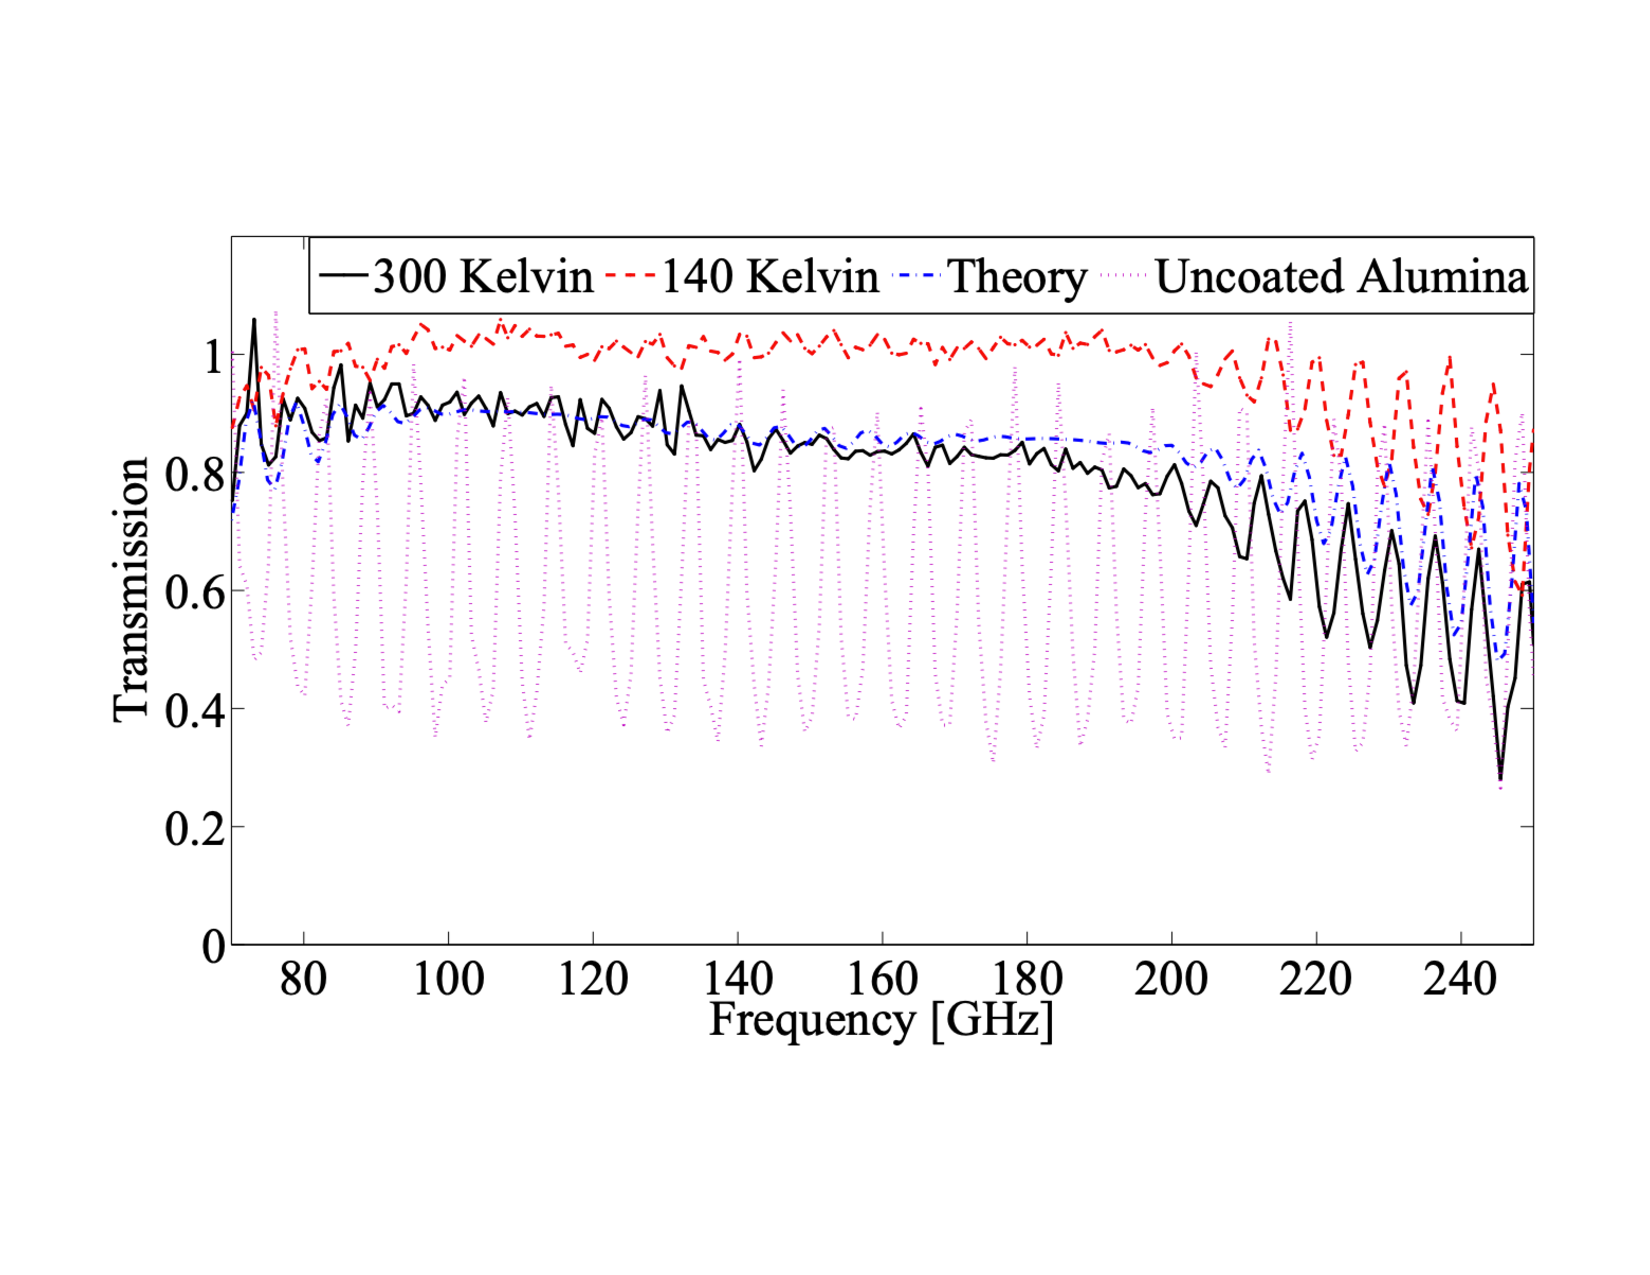
\includegraphics[width=0.7\linewidth, trim=1.5cm 3.5cm 1cm 3cm, clip]{ARCoating/Figures/epoxy_ar_measured.pdf}
    \caption{Measured performance of the epoxy AR coating on a 50~mm-diameter, 3~mm-thick alumina sample at both 300~K and 140~K. While the epoxy coating is lossy at room temperature, is emissivity decreases substantially at cryogenic temperatures. The measured fractional bandwidth is $\approx$~65\%, which is wide enough to cover PB-2a/b's 90 and 150~GHz bands.}
    \label{fig:measured_epoxy_ar_performance}
\end{figure}

In part because epoxy can be molded to a surface and in part because of the epoxy coating's excellent cryogenic performance as measured on a 50~mm-diameter sample, PB-2a selected the epoxy + epoxy AR coating for its lenses' curved surfaces. The process of applying 2850FT + 1090 to full-scale alumina optics was adopted from a procedure developed at Stanford for BICEP Array~\cite{Hui2018BICEPPolarimeter}, and the curved surfaces of the PB-2a lenses were coated at UC Berkeley between between 2014 and 2016. The flat sides of the PB-2a lenses were coated at the High Energy Research Organization (KEK) in Japan using a bottom layer of thermal-sprayed mullite and a top layer of an expanded polyimide foam called Skybond. For more information about the Mullite + plastic AR combination, see Section~\ref{sec:sapphire_ar_coating_mullite_duroid}. 

The AR coated PB-2a lenses were not measured directly, as taking the spectrum of a large object at cryogenic temperatures requires dedicated infrastructure that is both time-consuming and expensive to develop. Instead, they were installed in the PB-2a receiver cryostat and the band-averaged optical throughput of the full instrument was measured in the lab at KEK. In addition, the receiver's near-field beam was mapped in the lab to assess the roundness and angular extent of the optical response from detectors across the focal plane. The results of these tests were satisfactory for deployment, and therefore the PB-2a epoxy coatings were deemed a success~\cite{Kaneko2020DeploymentPolarbear-2A}. In order to leverage the work done for PB-2a, PB-2b adopted epoxy coatings for \textit{all} of its alumina and sapphire surfaces, both curved and flat, and the CHWP sapphire was part of the PB-2b AR-coating campaign. In the following sections, we review the epoxy coating process and the results of its application to sapphire.

%%%%%%%%%%%%%%%%%%%%%%%%%%%%%%%%
%%%%%%%%%%%%%%%%%%%%%%%%%%%%%%%%

\subsection{Fabrication}
\label{sec:sapphire_ar_coating_epoxy_fabrication}

The overall process for applying the epoxy + epoxy coating is
\begin{enumerate}
    \item Prepare the substrate.
    \item Mold Stycast 2850FT onto the substrate's bare surface.
    \item Mill the 2850FT layer to the target thickness.
    \item Mold Stycast 1090 onto the machined 2850FT layer.
    \item Mill the Stycast 1090 layer to the target thickness.
    \item Strain relieve the layers.
    \item Thermal cycle to cryogenic temperatures and inspect for mechanical degradation.
\end{enumerate}
We describe each of these steps in the following subsections, highlighting advancements made for PB-2b CHWP.

%%%%%%%%%%%%%%%%%%%%%%%%%%%%%%%%

\subsubsection{Surface preparation}
\label{sec:sapphire_ar_coating_epoxy_fabrication_surface_preparation}

The first step is to roughen the sapphire's surface. Aluminum oxide, of which both sapphire (single-crystal) and alumina (polycrystalline) are composed, is inert and does not easily bond to organic compounds. Therefore, a mechanical bond between the sapphire and epoxy, or one in which the epoxy flows into and ``grabs'' microscopic crevices in the substrate's surface, is critical to robust adhesion. As manufactured, the sapphire's surface has an RMS roughness of $\sim$~0.1~$\mathrm{\mu m}$ (see Figure~\ref{fig:sapphire_photo}), which auxiliary tests have shown to be insufficient for a robust epoxy-to-sapphire bond. Therefore, we roughen the surface ourselves\footnote{Metal Fusion: https://www.metalfusioninc.com/} before coating it.

\begin{figure}[!t]
    \centering
    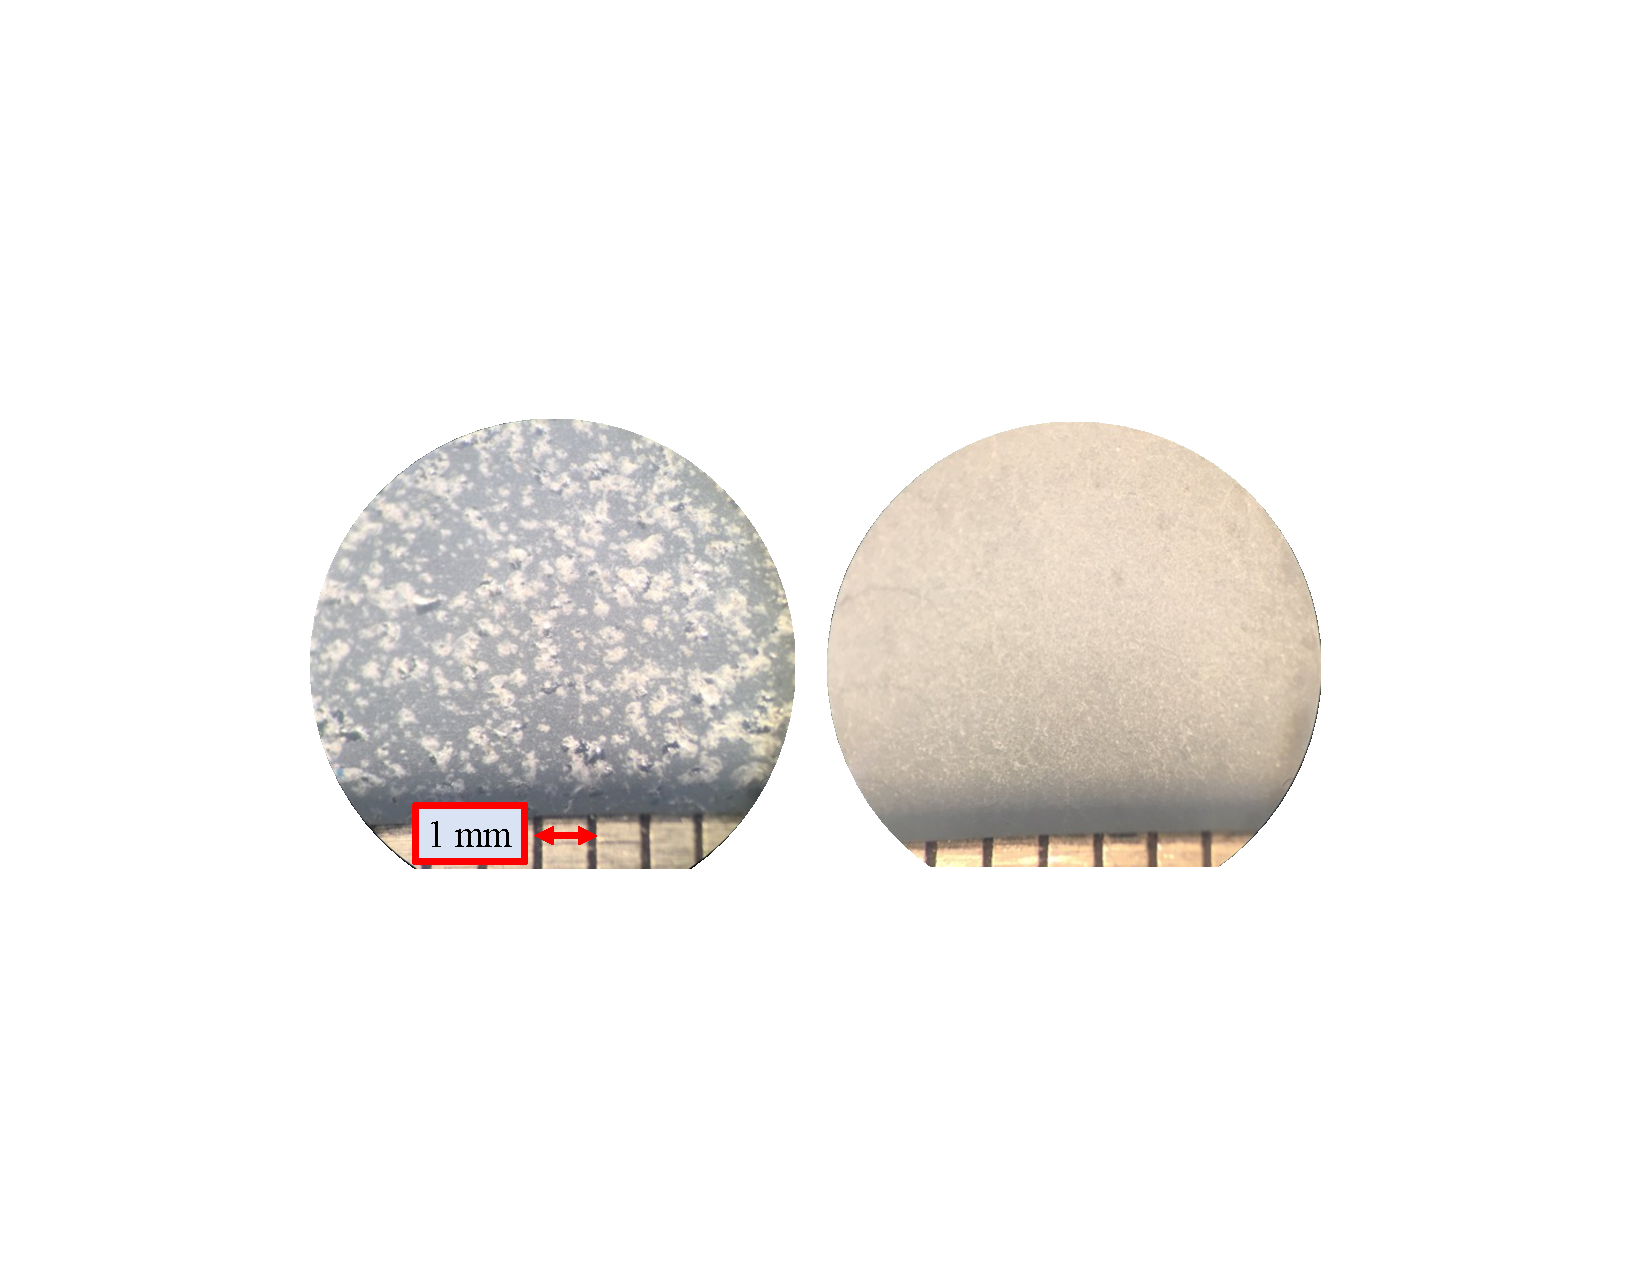
\includegraphics[width=0.7\linewidth, trim=5cm 6.5cm 5cm 6.5cm, clip]{ARCoating/Figures/sapphire_roughening.pdf}
    \caption[A microscope comparison of the sapphire surface after sandblasting vs. after sanding.]{A microscope comparison of a sapphire surface after 24-grit sandblasting at 50 PSI (left) and of a different sapphire surface after abrating with 60-grit diamond sandpaper (right). The sandblasting cracks the sapphire at its surface, making it vulnerable to fracture, while the sanding roughens the surface without any visible damage.}
    \label{fig:sapphire_roughening}
\end{figure}

While PB-2a found sandblasting to be adequate for robust epoxy adhesion to alumina, sapphire requires a more nuanced abrasion approach. Figure~\ref{fig:sapphire_roughening} shows a comparison of a sapphire surface that has been sandblasted with 24-grit silicon carbide vs. a surface that has been sanded with 60-grit diamond sandpaper. As is evident in the photo, sandblasting introduces microcracks beneath the surface, and this subsurface damage makes the sapphire vulnerable, as these microcracks can propagate when stressed upon cooling. For this reason, we instead sand the surface using diamond sandpaper, making sure to roughen both evenly and gently. 

\begin{figure}[!t]
    \centering
    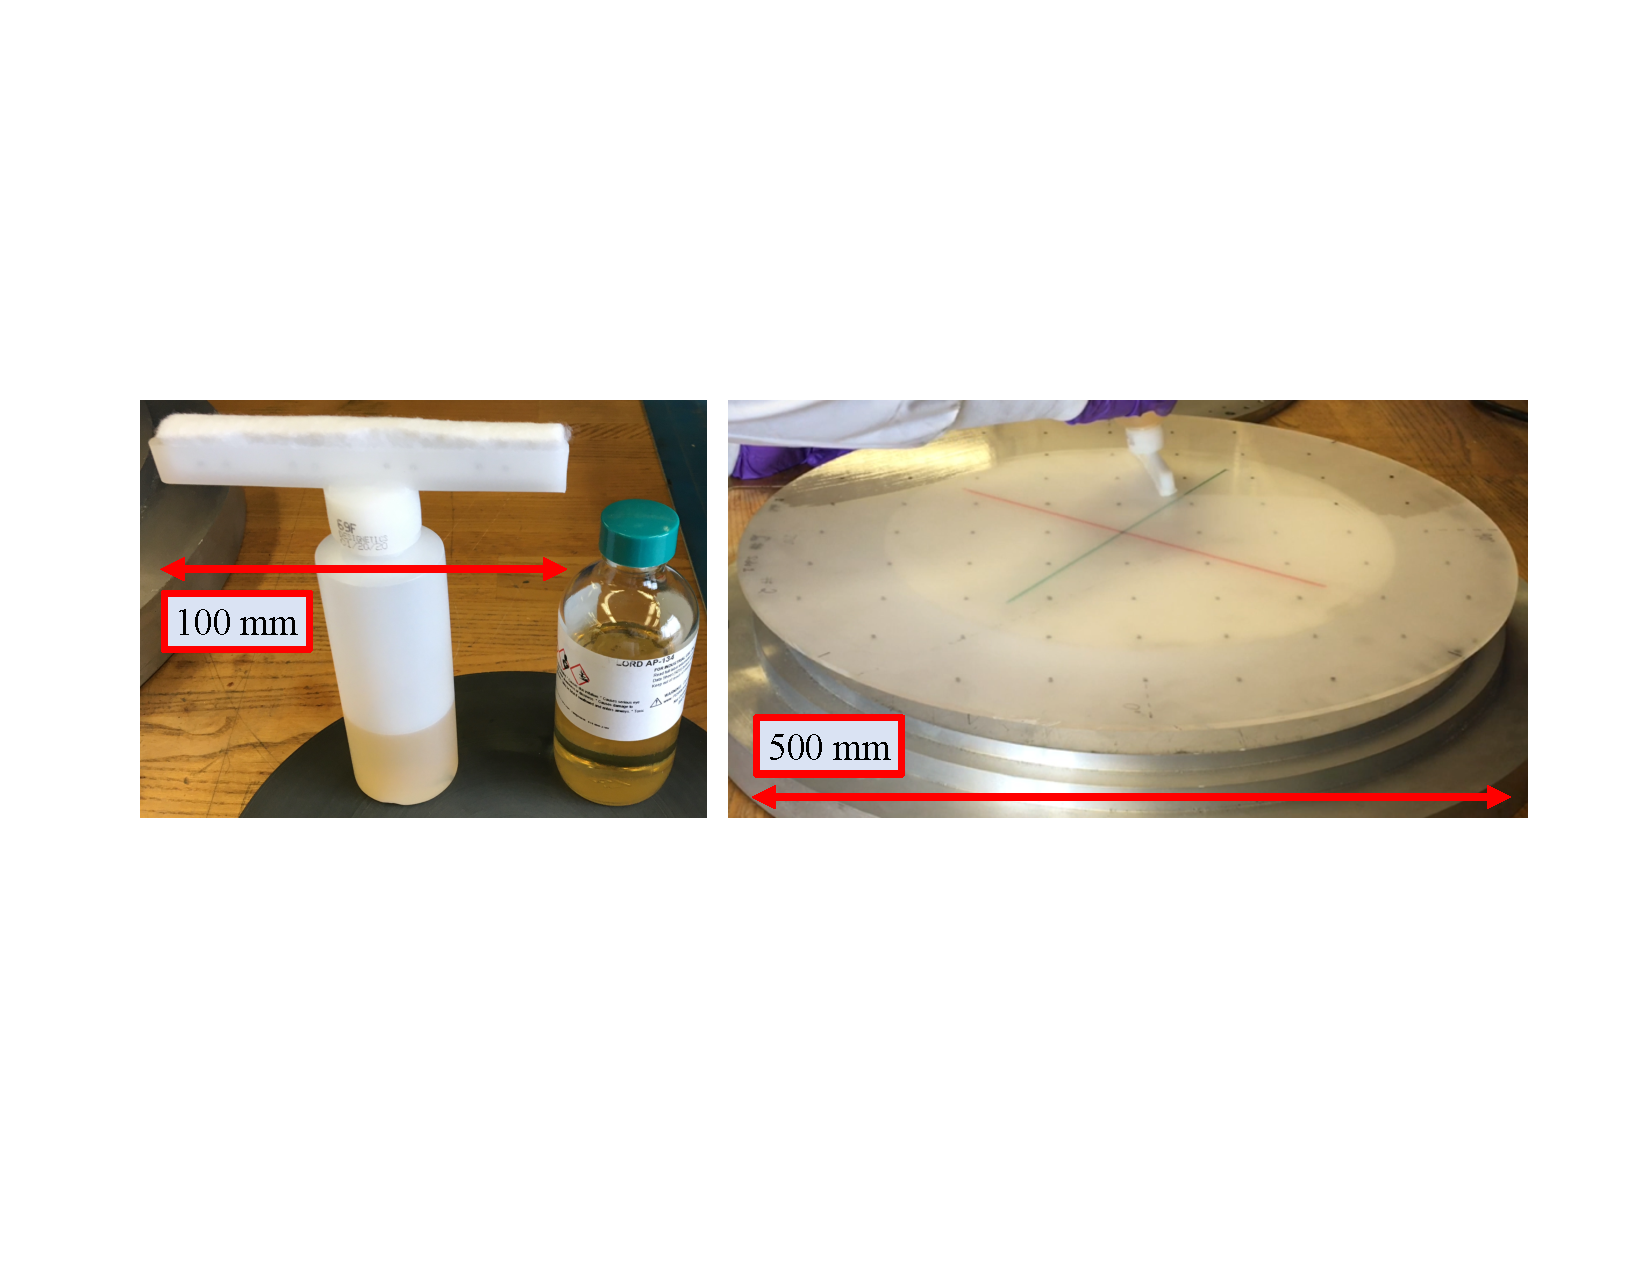
\includegraphics[width=\linewidth, trim=2cm 7.5cm 2cm 6cm, clip]{ARCoating/Figures/sapphire_ap_application.pdf}
    \caption[Photos of the upgraded AP-134 application technique used for the PB-2b sapphire.]{Photos of the AP-134 application technique used for the PB-2b sapphire. The photo on the left shows a bottle of AP-134 (right) next to the felt applicator tip (left) used to apply it. The photo on the right is a snapshot of the application process. The tip and its bottle are flipped upside-down, the bottle is squeezed, and the solution soaks the felt. Then AP-134 is then ``painted'' onto the sapphire, and its dispensation rate is controlled by how hard the tip is pressed against the surface.}
    \label{fig:sapphire_ap_application}
\end{figure}

After the surface is roughened, we clean it thoroughly using Scotch-Brite\footnote{Scotch-Brite: https://www.scotch-brite.com/3M/en\_US/scotch-brite/} and solvents, and we apply a thin film of Lord AP-134 adhesion promoter.\footnote{Lord AP-134: https://www.lord.com/products-and-solutions/chemlok-ap-134-primer} AP-134 is a ceramic-compatible primer that allows the epoxy to bond \textit{chemically} to the sapphire and consists of an organosilane dissolved in solvents. When the primer is applied to the sapphire's surface, the solvents quickly evaporate off, and the organosilane hydrolyzes and bonds to dangling hydroxyl groups on the substrate. This curing process sets up a stout, crosslinked silane network with free-radial groups that the epoxide molecules can now bond to. The success of the adhesion promoter relies on the applied AP-134 layer being thin and even and on the silane network being sufficiently hydrolyzed. Prior to PB-2b epoxy development, the primary technique to apply AP-134 was to dab a Kimwipe in the solution and wipe it across optic's surface. Because this process has no thickness control, PB-2b uses felt applicator tips from Designetics\footnote{Designetics: https://designetics.com/} to provide a thinner, more even coverage. The AP layer is left to hydrolyze for 2$\sim$3 hours at 50$\sim$80\% humidity\footnote{If the ambient humidity is less than 50\%, as often happens during the summertime in Berkeley, then the cure time is extended appropriately.} before the coating process advances. Figure~\ref{fig:sapphire_ap_application} shows an applicator tip as well as the adhesion promoter being applied to the surface. After hydrolyzation is complete, the cured adhesion promoter leaves a hazy finish whose uniformity can be verified by eye.

%%%%%%%%%%%%%%%%%%%%%%%%%%%%%%%%

\subsubsection{Coating}
\label{sec:sapphire_ar_coating_epoxy_fabrication_coating}

After the sapphire surface is prepared, the Stycast 2850FT must be mixed and applied. We note that the application of the 1090 top layer follows a nearly identical procedure, and therefore this section describes steps 2 and 4 of the fabrication process. The most important goals of the Stycast application is to achieve a thin, uniform layer free of air bubbles.\footnote{Voids act as mm-wave scatterers, which can substantially reduce the AR coating's transparency. We do not have an air-bubble requirement for PB-2b, but a good ``rule of thumb'' to achieve negligible loss 150~GHz is for all bubbles to be $<$~100~$\mathrm{\mu m}$ and to be sparsely populated.}

First, to ensure that the fillers are evenly distributed throughout the epoxy, we warm the resin alone up to $\approx$~$40^{\circ}$~C to reduce its viscosity and mix it in the can using a hand drill and an aluminum paddle for $\approx$~5~min, as shown on the left side of Figure~\ref{fig:epoxy_curing}. This step is especially important when using a fresh can, as the fillers may sink/float to the bottom/top of the resin within its shelf life. After the resin cools to $<$~$30^{\circ}$, we extract $\approx$~700~g of 2850FT and mix it with $\approx$~50~g of Catalyst 23LV by hand for $\approx$~5~min or until the color of the mixture is even. We then evacuate the mixture down to $\approx$~3~Torr over 8~min using a high-throughput roughing pump, removing trapped air. The evacuation step has been tuned carefully, as pumping for too long can cause the mixture to overheat and pumping for too little results populations of $>$~0.1~mm air bubbles throughout the AR layer.

\begin{figure}[!t]
    \centering
    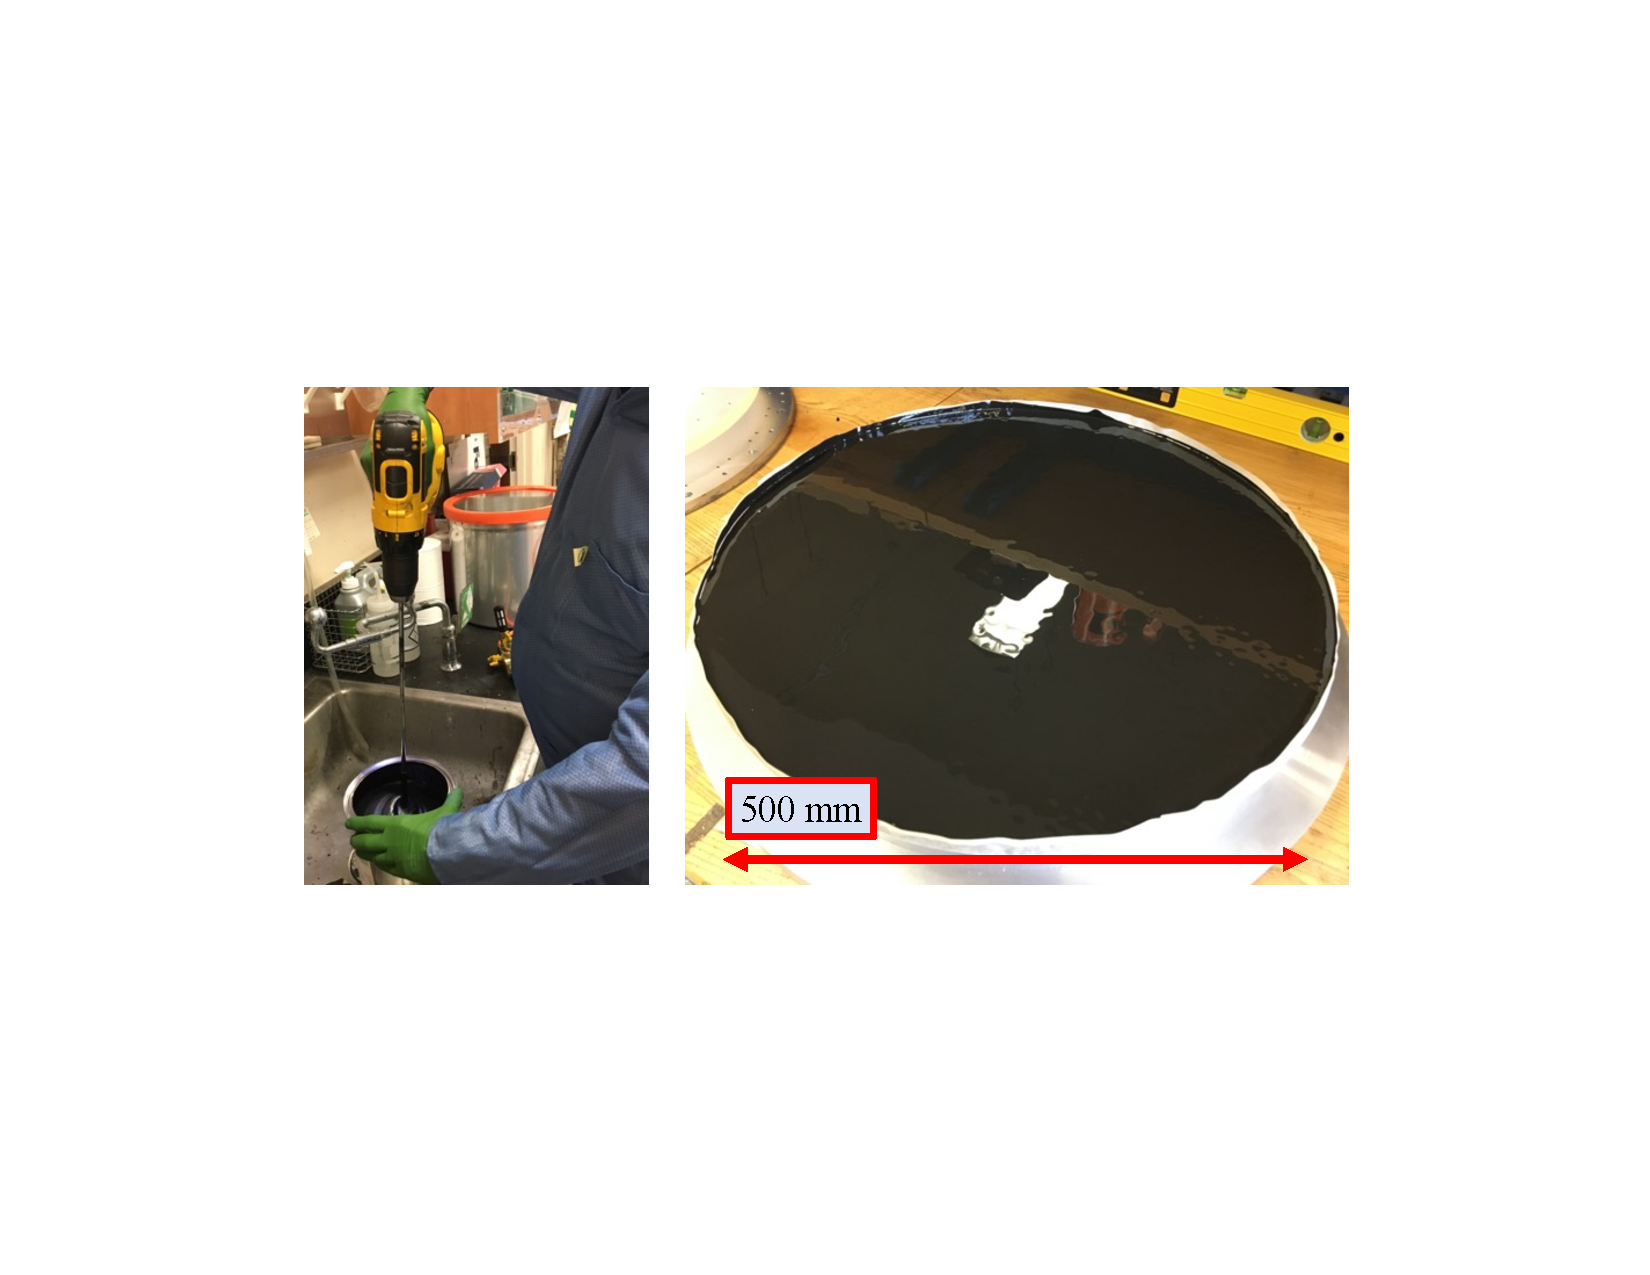
\includegraphics[width=0.7\linewidth, trim=5cm 6.5cm 5cm 6.5cm, clip]{ARCoating/Figures/epoxy_curing.pdf}
    \caption[Photos of the epoxy AR application and cure.]{Photos of the epoxy AR application and cure. The left photo is of the epoxy resin being mixed in the can, which is important to distribute the fillers evenly. The right photo is of the epoxy mixture on the sapphire surface right after application. It is coated all the way to the edge, and a barrier of masking tape keeps it the epoxy from leaking over the edge. A leveling table keeps the layer flat which it cures over 24 hours.}
    \label{fig:epoxy_curing}
\end{figure}

After the epoxy is mixed and evacuated, it is monitored using an IR thermometer until its temperature is $>$~$30^{\circ}$~C.\footnote{The act of evacuating the epoxy mixes it further, and because the epoxy reaction is exothermal and because the mixture is in a vacuum space, it can warm substantially during the 8-minute pump.} It is important to control the epoxy's temperature throughout the mixing process as epoxide catalysis is an exothermal chemical reaction where temperature increases  accelerate the cure and hence make the epoxy more difficult to handle. Once the epoxy is cool enough, it is slowly poured into a blob on the center of the sapphire surface, and the part is rotated such that gravity spreads the mixture towards the edges. After the surface is fully coated, it is stored on a leveled surface to cure for 24 hours in ambient conditions.

In addition to coating the surface, for each 2850FT and 1090 layer we put down, we measure a 50~mm-diameter by $\approx$~20~mm-thick witness sample to determine the layer's refractive index. Fluctuations in index arise due to fluctuations in filler fraction, and we find that variations in both $n_{\mathrm{2850FT}}$ and $n_{\mathrm{1090}}$ can be as large as 5\% between batches.\footnote{The manufacturing batch number is printed on the front of each can of resin.} Because the ideal thickness for the coating is tied to its refractive index (see Equation~\ref{eq:lambda_over_four_thickness}), this index verification is central to minimizing reflectivity during the fabrication process.

%%%%%%%%%%%%%%%%%%%%%%%%%%%%%%%%

\subsubsection{Machining}
\label{sec:sapphire_ar_coating_epoxy_fabrication_machining}

\begin{figure}[!t]
    \centering
    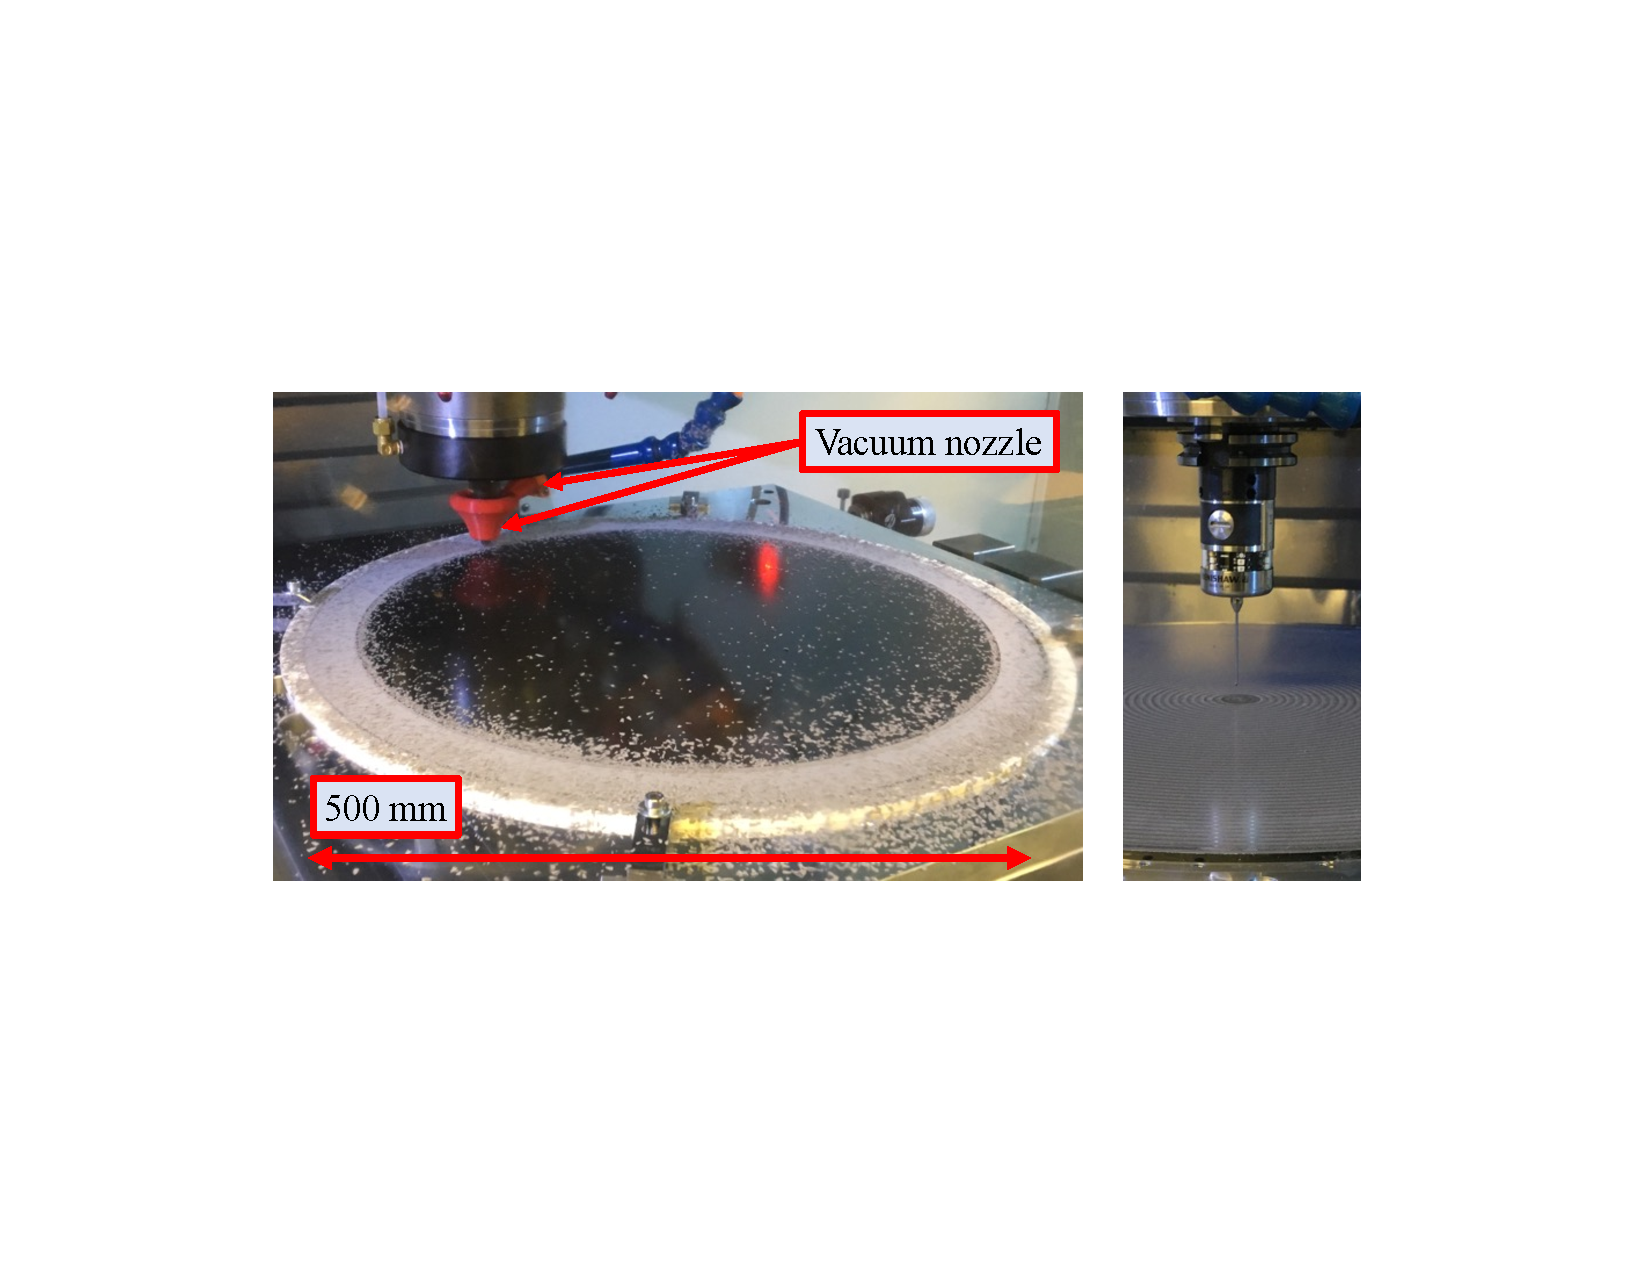
\includegraphics[width=\linewidth, trim=4cm 6.5cm 4cm 6.5cm, clip]{ARCoating/Figures/epoxy_machining.pdf}
    \caption[Photos of epoxy AR coating machining and metrology.]{Photos of epoxy AR coating machining and metrology. The left photo shows a roughing cut on a cured 2850FT layer. The roughing cut is followed by a pre-finish cut to check for any $z$-offsets caused by end-mill wear or spindle expansion, and the finish cut ``skims'' to the target thickness. The photo on the right shows the Renishaw contact probe used to measure both the bare optic surface before the epoxy is cured and of the the epoxy surface after machining.}
    \label{fig:epoxy_machining}
\end{figure}

After the epoxy layer has cured, we next machine it to its target thickness. We use a vacuum chuck to fix the piece in a Haas VM3\footnote{Haas VM3: https://www.haascnc.com/machines/vertical-mills/mold-machines/models/vm-3.html} computer numerical controlled (CNC) mill, and we use a diamond-coated end mill to machine the epoxy. The diamond-coated bit is necessary because the fillers in both epoxies are abrasive and wear down tooled steel or silicon carbide bits. Stycast particles are hazardous to breathe, and therefore care is taken to ventilate any dust generated during machining using a vacuum nozzle coupled to a high efficiency particulate air (HEPA) filter. 

Because the tolerance on the layer's thickness is tight, it is critical to control the spindle height throughout the machining process, which in turn relies on control of the machine's temperature. The UC Berkeley physics machine shop is currently not temperature controlled,\footnote{Temperature control for the physics machine shop is in the facilities manager's upgrade queue.} and therefore scheduling machining cycles during times of stable ambient temperature\footnote{For example, we typically perform finish cuts during the afternoon as opposed to during the morning, and we are wary about working during especially hot days.} is important to avoiding thickness gradients. In addition, we find that the spindle length slowly increases by $\sim 100$~$\mathrm{\mu m}$ during the first $\sim$hour after it is started. Therefore, we run an $\sim$hour-long ``warm-up'' cycle prior to each epoxy cut, after which we use gauge blocks to measure any spindle elongation and correct the target $z$-dimension accordingly. To minimize the impact of additional spindle elongation during the machining cycle, we use a somewhat aggressive stepover to keep the cycle time to $\lesssim$~1~hour.

After the warm-up cycle, we machine the epoxy layer in three steps: a rough cut to remove the majority of the excess material, a pre-finish cut to cross-check and calibrate the cutter's $z$-dimension, and the finish cut. After each of these cycles, the surface is probed using a Renishaw contact probe\footnote{Renishaw OMP400: https://www.renishaw.com/en/omp400-high-accuracy-machine-probe--6089} with a 1~mm-diameter ruby tip. We probe four points at three different diameters in addition to at the center, and these thirteen measurements are differenced to an identical measurement of the bare sapphire surface---or in the case of the 1090 top layer, a measurement of the machined 2850FT bottom layer---to extract both the layer's overall thickness and its uniformity. This machining and metrology procedure has proven to reliably meet our $\pm$~$25$~$\mathrm{\mu m}$ tolerances.

It sometimes happens that air bubbles within the cured epoxy layer will appear during the machining process, and these voids need to filled. Therefore, after the pre-finish cut, which is typically $\approx$~$125$~$\mathrm{\mu m}$ over the target thickness, we mix a small amount of epoxy, roughen the cavities using a steel brush, and fill them in place on the mill. These patches are then left to cure overnight before proceeding to the finish cut.

%%%%%%%%%%%%%%%%%%%%%%%%%%%%%%%%

\subsubsection{Strain relieving}
\label{sec:sapphire_ar_coating_epoxy_fabrication_strain_relief}

After both the 2850FT and 1090 layers have been applied and machined, the sapphire is \textit{technically} coated, and if the HWP operated at ambient temperature, we would at this point be finished. However, there are substantial differences between the CTEs of the epoxy AR coating and the sapphire substrate, and therefore we must strain relieve the coating to avoid delamination when cooling the CHWP to 50~K. 

As was done for the PB-2a optics, we \important{laser dice} the epoxy at Laserod.\footnote{Laserod: https://laserod.com/} Laserod uses an ultraviolet 355~nm, $\sim$~10~W, nanosecond-pulse laser to cut all the way to the sapphire substrate, separating the AR coating into detached \important{islands}. The UV wavelength is necessary to achieve a $\lesssim$~30~$\mathrm{\mu m}$ kerf, which is required to avoid polarized diffraction induced by the strain-relief cuts. Also following the findings of PB-2a, we dice with a 1~cm pitch along two orthogonal directions, which separates the epoxy layer into a grid of 1~cm~$\times$~1~cm square pieces. To calibrate the depth of cut, the machinist monitor's the sapphire's semi-transparent backside for laser light to peek through the epoxy-substrate interface and appends $\sim$~10\% additional passes to ensure complete separation. Verifying complete separation is particularly important, as it was found during both PB-2a that \important{incomplete dicing} leads to widespread delamination upon cooling.

\begin{figure}[!t]
    \centering
    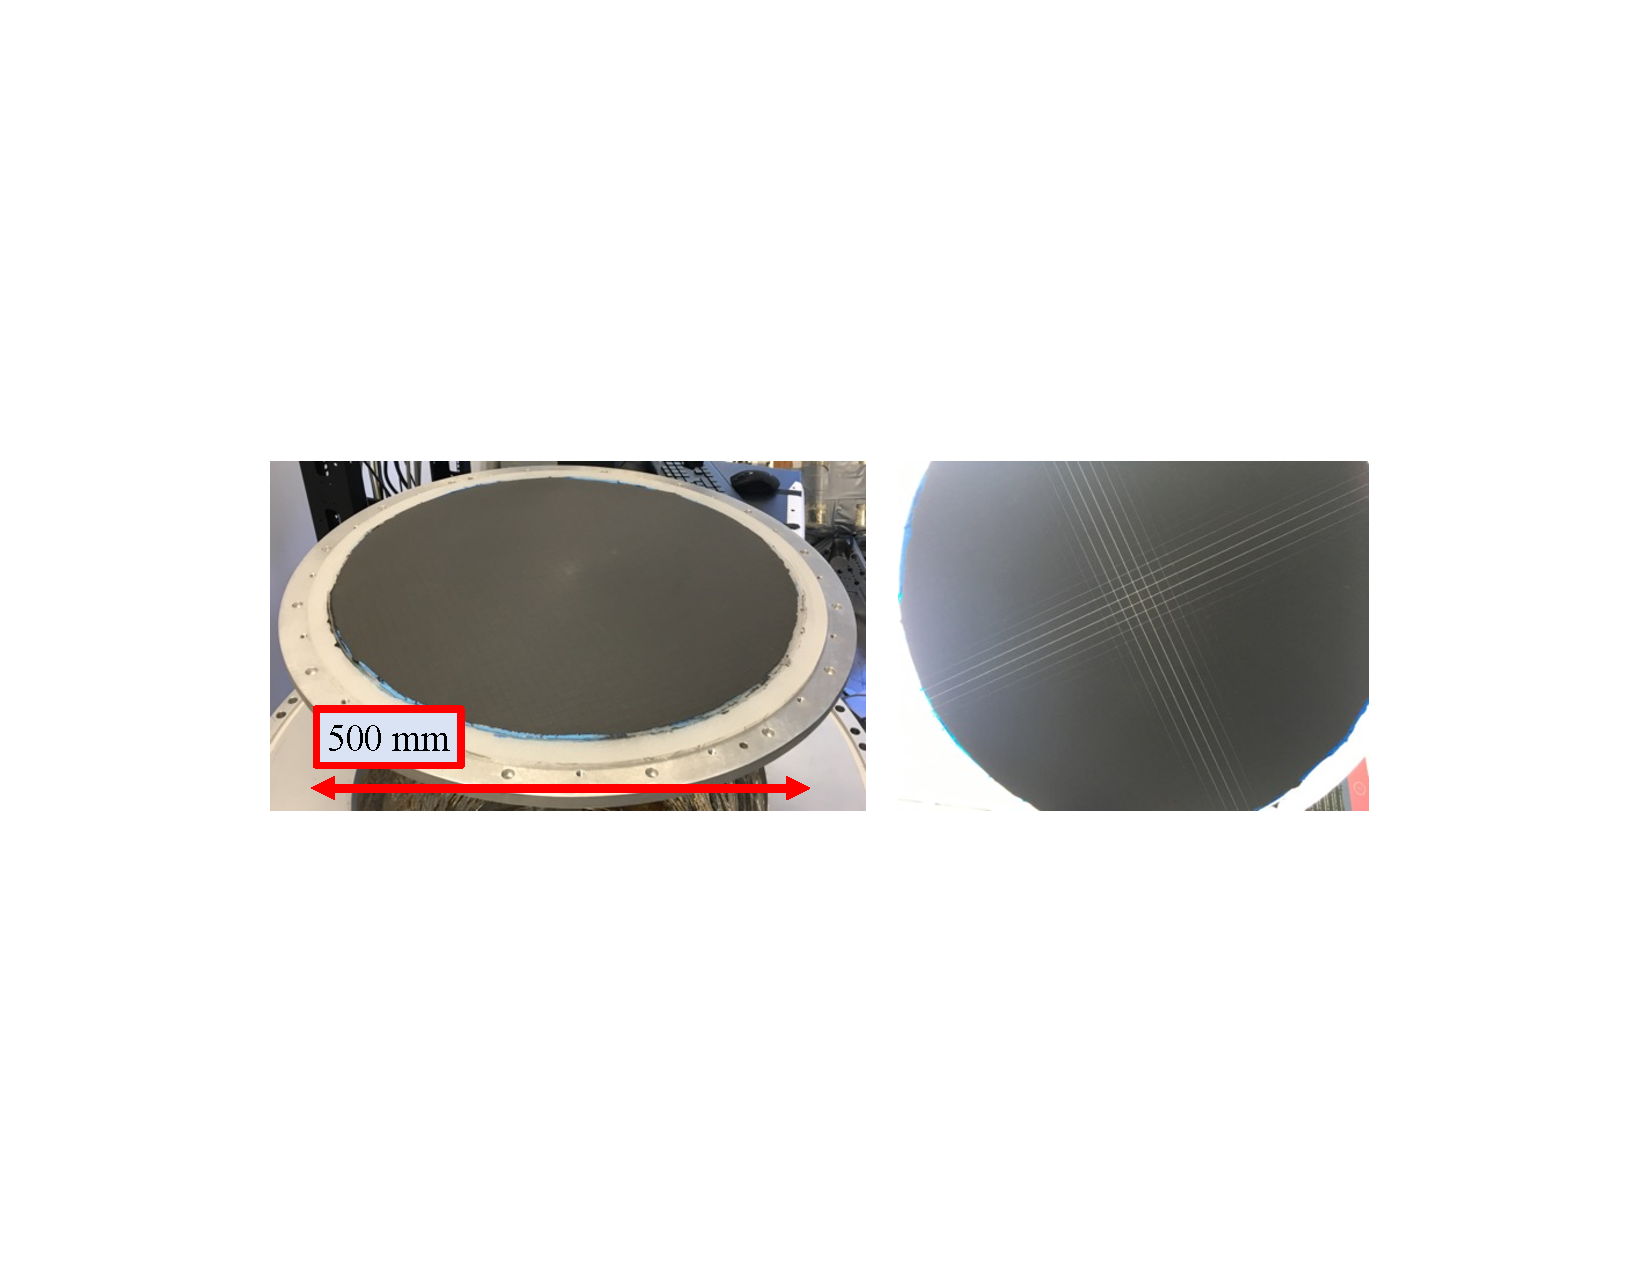
\includegraphics[width=\linewidth, trim=4cm 8cm 4cm 7.5cm, clip]{ARCoating/Figures/sapphire_epoxy_ar_before_cooling.pdf}
    \caption[Photos of the epoxy-coated sapphire after fabrication and before thermal cycling.]{Photos of the epoxy-coated sapphire after fabrication and before thermal cycling. The photo on the left shows the fully fabricated epoxy AR coating on a 20" sapphire window mounted in the CAPMAP dewar prior to thermal cycling. The faint 1~cm~$\times$~1~cm lines are the strain relieving laser cuts. The photo on the right is that same piece held with its bare backside to the window, showing that the dicing lines cut all the way through the AR coating and verifying that each 1~cm~$\times$~1~cm island will contract independently when cooled.}
    \label{fig:sapphire_epoxy_coated_before_cooling}
\end{figure}

Additional investigations of the laser dicing process were performed to better understand how the epoxy is ablated, how the heat-affected zone changes with pulse duration, and how overdicing impacts the mechanical strength of the sapphire, but these investigations were part of the epoxy + Duroid AR campaign and are therefore discussed in Section~\ref{sec:sapphire_ar_coating_epoxy_plastic}.

%%%%%%%%%%%%%%%%%%%%%%%%%%%%%%%%

\subsubsection{Thermal cycling}
\label{sec:sapphire_ar_coating_epoxy_fabrication_thermal_cycle}

The final step of the fabrication process is to validate cryo-mechanical performance. As demonstrated by Figure~\ref{fig:measured_epoxy_ar_performance}, the optical constants of 2850FT and 1090 are largely consistent with temperature, and the coating's transmissivity is excellent on a 50~mm-diameter at cryogenic temperatures. Therefore, the primary purpose of this final step is to assess the AR coating's adhesion on a full-scale sapphire piece after laser dicing.

The fully coated sapphire is cooled to $\approx$~20~K and warmed back to $\approx$~300~K over $\approx$~48~hours using a Gifford-McMahon (GM) cooler in the CAPMAP dewar at Lawrence Berkeley National Laboratory (LBNL). After the piece is returned to ambient conditions, its surface is inspected for any delaminated epoxy islands, and the adhesion layer is inspected through the sapphire's semi-transparent backside. If substantial damage is found, then the fabrication process is, in most cases, considered to be unsuccessful. On the other hand, if the quality of adhesion looks unaffected by the thermal cycle, then the CAPMAP cooldown is repeated several more times to check the coating's robustness to multiple stress cycles. If the piece survives this gauntlet of cryogenic testing, then it is qualified for optical use. 

Note that we do not measure each full-scale sapphire piece, as doing so at cold temperatures requires dedicated, expensive infrastructure. Instead, we use index measurements of the witness pieces and thickness measurements of the machined layers to calculate the expected performance of each piece. This technique is a valid approximation of the realized performance in the absence of mechanical degradation.

%%%%%%%%%%%%%%%%%%%%%%%%%%%%%%%%
%%%%%%%%%%%%%%%%%%%%%%%%%%%%%%%%

\subsection{Performance}
\label{sec:sapphire_ar_coating_epoxy_peformance}

In this section, we consider two performance metrics for the epoxy AR coating: reflectivity at low temperatures and cryo-mechanical robustness. Because a comparison of the epoxy coating's warm and cold transmissivity has already been published on a 50~mm-diameter, un-diced piece, we in this section focus on the performance of larger-diameter, diced parts, which are most representative of deployable optics. We will discuss the cryo-mechanical performance first, as doing so best sets the stage for a discussion of optical performance.

%%%%%%%%%%%%%%%%%%%%%%%%%%%%%%%%

\subsubsection{Cryo-mechanical performance}
\label{sec:sapphire_ar_coating_epoxy_cryo_mechanical_performance}

The primary differences between small-scale epoxy coatings, which have been characterized and published, and full-scale epoxy coatings, which have not, are the coating diameter and the laser strain relieving. Therefore, the dominant mechanism though which the optical performance of large pieces could degrade in a way not seen on smaller pieces is through \important{cryogenic delamination}, or separation of the AR coating away from the optical substrate upon cooling to low temperatures. For this reason, assessing cryogenic robustness is the first step of the evaluation process. If the cryogenic robustness is deemed to be adequate, then it is reasonable to assert that the performance of small-scale pieces will represent that of full-scale pieces.

\begin{figure}[!t]
    \centering
    \subfloat[\label{fig:epoxy_delamination:a}]{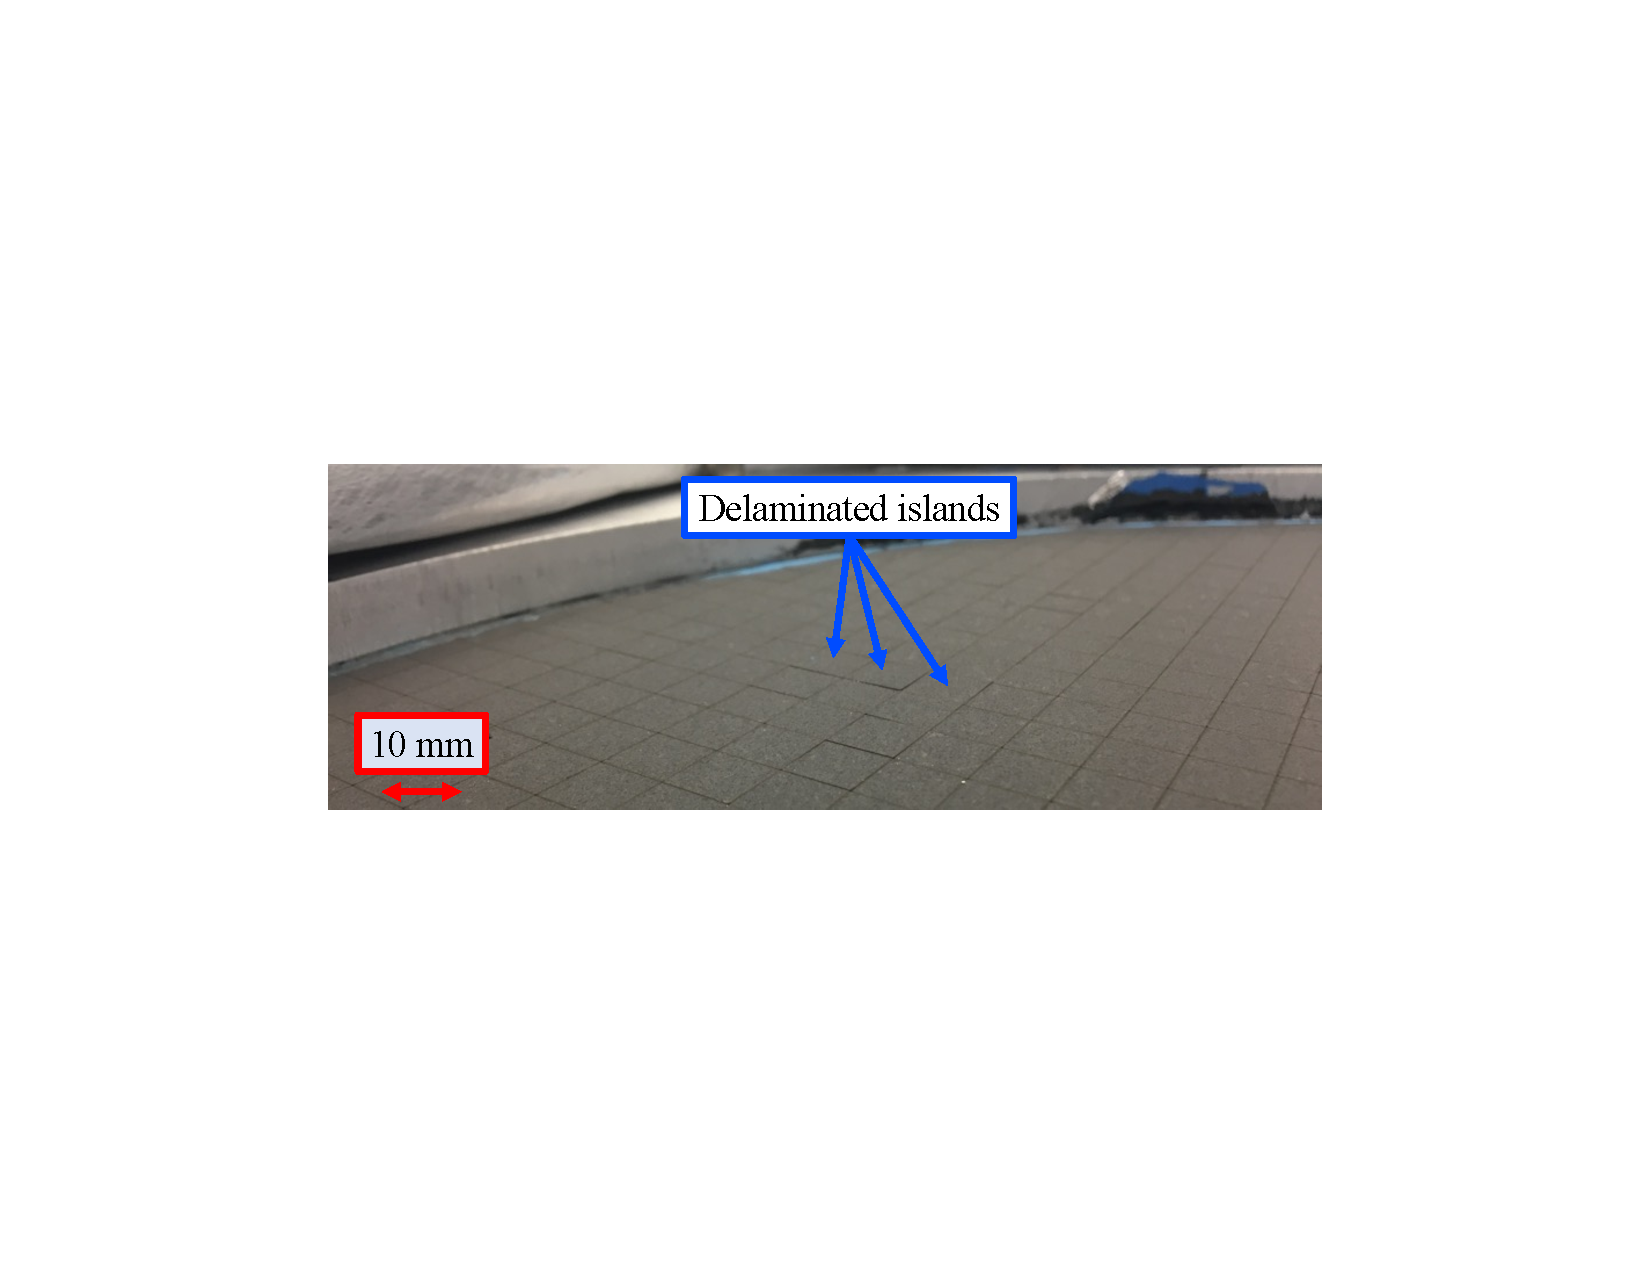
\includegraphics[width=0.8\linewidth, trim=4cm 7.5cm 4cm 7.5cm, clip]{ARCoating/Figures/epoxy_delaminated_islands.pdf}}
    \hfill
    \subfloat[\label{fig:epoxy_delamination:b}]{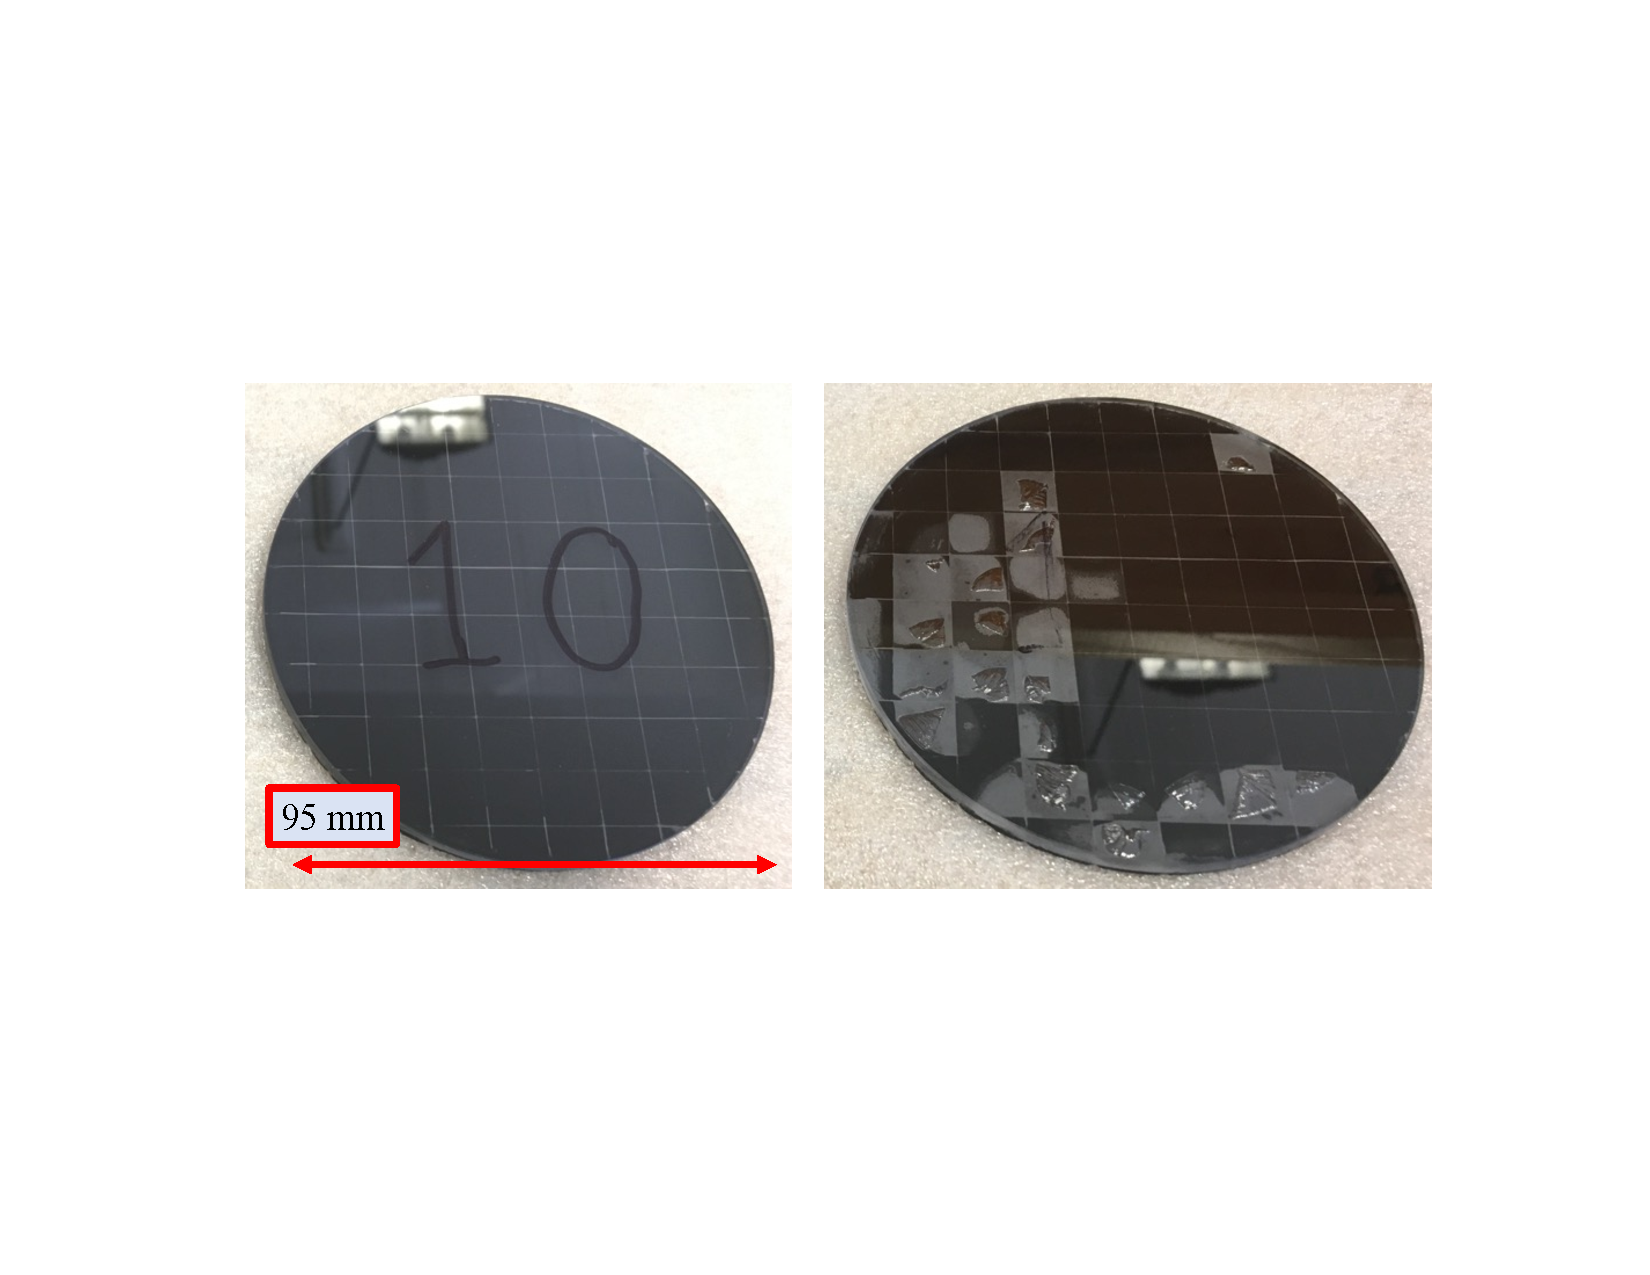
\includegraphics[width=0.7\linewidth, trim=4cm 6cm 4cm 6cm, clip]{ARCoating/Figures/epoxy_delamination_test_piece.pdf}}
    \caption[Photos of cryogenic delamination of Stycast 2850FT + Stycast 1090 on sapphire.]{Cryogenic delamination of Stycast 2850FT + Stycast 1090 on sapphire. The top photo shows the result of one cooldown of the 500~mm-diameter piece shown in Figure~\ref{fig:sapphire_epoxy_coated_before_cooling}. Some epoxy squares that have partially delaminated when cold did not fully flatten after warming and therefore show a raised edge at the laser groove. The bottom picture shows a followup test on a 95~mm, polished sapphire piece as viewed through the transparent backside before (left) and after (right) cooling. Grey areas indicated AR separation, while shimmering patches indicate fractured sapphire.}
    \label{fig:epoxy_delamination}
\end{figure}

Figure~\ref{fig:epoxy_delamination} shows the result of thermal cycling a 500~mm-diameter piece as well as that of thermal cycling a 95~mm-diameter piece. Even though sanding the surface damages it less than sandblasting, the epoxy pulls ``chunks'' out of the substrate as a result of the epoxy contracting more than sapphire upon cooling. We also note that while this delamination only occurs in some areas, it progresses with each cooldown and therefore affects a larger fraction of the surface over time.

%%%%%%%%%%%%%%%%%%%%%%%%%%%%%%%%

\subsubsection{Optical performance}
\label{sec:sapphire_ar_coating_epoxy_optical_peformance}

As discussed in the previous section, the epoxy AR coating breaks the sapphire substrate upon cooling. While this result may appear to preclude the epoxy AR coating from consideration, we use an optical measurement to check two things: what the impact of this delamination is on optical performance, and whether this same effect occurs on alumina. Therefore, we coat a 150~mm-diameter, 3~mm-thick piece of alumina and measure it in a reflectometer at the University of Michigan.

\begin{figure}[!t]
    \centering
    \subfloat[\label{fig:epoxy_on_alumina_delamination:a}]{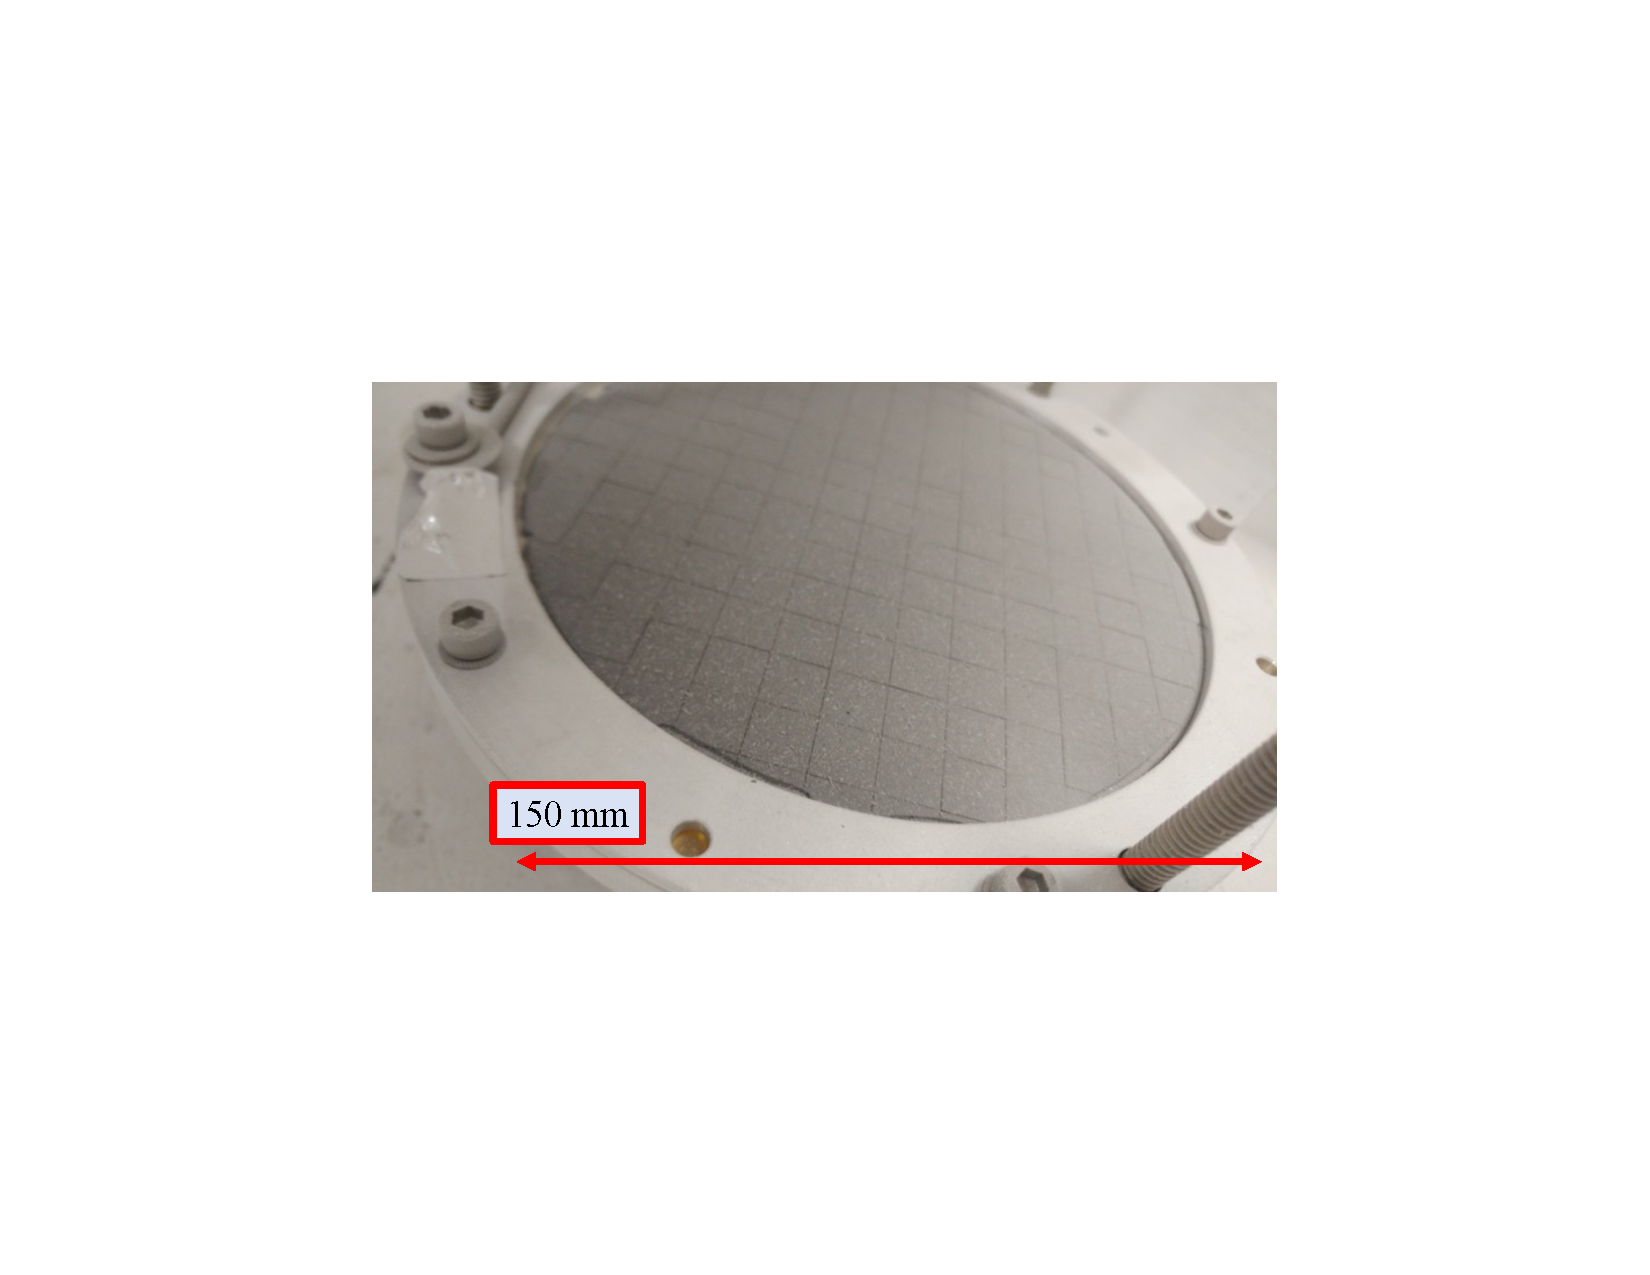
\includegraphics[width=0.48\linewidth, trim=5cm 4.5cm 5cm 5.5cm, clip]{ARCoating/Figures/epoxy_on_alumina_partial_delamination.pdf}}
    \subfloat[\label{fig:epoxy_on_alumina_delamination:b}]{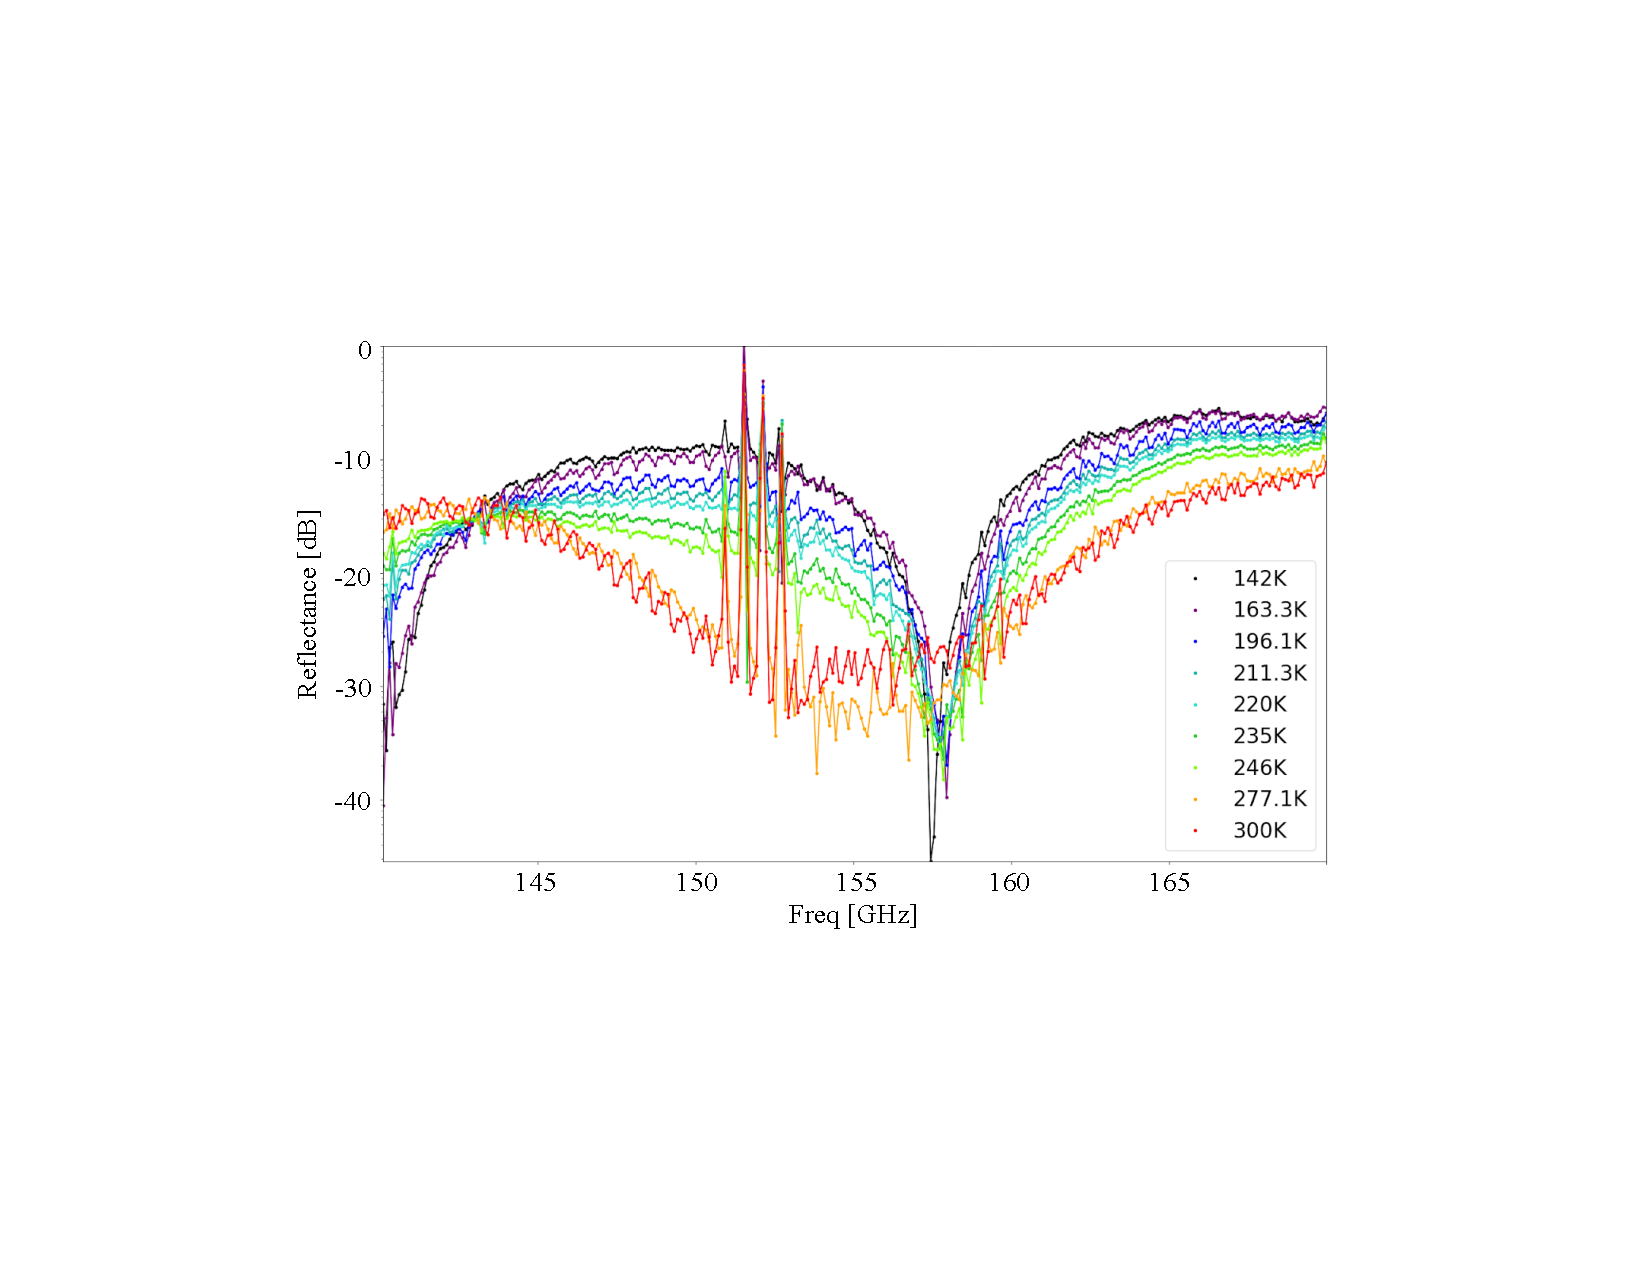
\includegraphics[width=0.48\linewidth, trim=5cm 5.5cm 5cm 5.5cm, clip]{ARCoating/Figures/epoxy_on_alumina_reflectance_measurement.pdf}}
    \caption[Partial delamination of epoxy from alumina and the resulting impact on reflectance vs. temperature.]{Partial delamination of epoxy from 6"-diameter alumina coated on both sides and the resulting impact on reflectance vs. temperature. Figure~\ref{fig:epoxy_on_alumina_delamination:a} shows that sample, connected to a liquid nitrogen bath, at $\approx$~140~K. The small icicles on the surface formed long after all measurements had finished. Figure~\ref{fig:epoxy_on_alumina_delamination:b} shows the resulting reflectance vs. temperature between 140$\sim$170~K. The increase in reflectance is reasonably well modeled by a non-uniform air gap of 50$\sim$100~$\mathrm{\mu m}$ developing between the sapphire and bottom 2850FT epoxy layer.}
    \label{fig:epoxy_on_alumina_delamination}
\end{figure}

Figure~\ref{fig:epoxy_on_alumina_delamination:a} is a photo of the alumina sample, coated on both sides, suspended over a bath of liquid nitrogen (LN2), and cooled to $\approx$~140~K. It's subtle to see, but the square islands are indeed raising at the dicing lines, and this partial delamination is creating an air gap between the bottom 2850FT epoxy layer and the alumina substrate. Measurements of reflectance between 140$\sim$170~GHz at various temperatures are shown in Figure~\ref{fig:epoxy_on_alumina_delamination:b}, and the influence of the air gap clearly increases reflectance with decreasing temperature temperature. This measurement was performed several times, and the result was shown to be repeatable.

%%%%%%%%%%%%%%%%%%%%%%%%%%%%%%%%
%%%%%%%%%%%%%%%%%%%%%%%%%%%%%%%%

\subsection{Assessment}
\label{sec:sapphire_ar_coating_epoxy_assessment}

The epoxy + epoxy AR coating of Stycast 2850FT + Stycast 1090 has several issues. Despite advancements in the coating technique, including more gentle surface roughening via sanding instead of sandblasting and a more uniform, repeatable adhesion-promoter layer, the AR coating separates from the sapphire substrate when cooled to cryogenic temperatures. In fact, the epoxy pulls chunks out of the substrate itself, as shown in Figure~\ref{fig:epoxy_delamination:b}, indicating that the combination of both the epoxy's large CTE and large tensile modulus may be too much for the sapphire to withstand. There are two clear solutions that could remedy this problem. The first solution is to laser dice more finely to shrink the isolated islands and hence reduce the stress due to differential contraction. While this modification is straightforward to implement, it is expensive\footnote{Machining time on Laserod's 355~nm laser is expensive, and the machining time scales as the square of the dicing pitch.} and would quickly make the epoxy AR process unaffordable. In addition, as we discuss in Section~\ref{sec:sapphire_ar_coating_epoxy_plastic_fabrication_5880LZ_strain_relieving}, laser dicing introduces its own complications that make it less obvious that finer dicing is better.

The second solution is to change the top layer. Successful cryo-mechanical tests of the 2850FT layer alone on 95~mm samples suggest that the 1090 layer is to blame for the observed delamination. Stycast 1090 both shrinks more quickly than 2850FT and is stiff at low temperatures, and therefore it has a propensity to \textit{peel} the bottom layer away from the substrate.\footnote{This peeling issue is much less of a problem for single-layer AR coatings, as in that case nearly all of the force due to differential thermal contraction is parallel to the surface where adhesion in strongest. For this reason among others, single-layer coatings are substantially simpler to implement for cryogenic applications, and the presented cryo-mechanical challenges are largely unique to multi-chroic coatings.} In addition, Stycast 1090's index has drifted higher over time, presumably due to changes in the epoxy's manufacturing,\footnote{We have reached out to Loctite several times about whether the filler concentration in Stycast 1090 may have decreased over the years, but the manufacturer assures us that the formula remains unchanged. Keith Thomson at Stanford has also seen the 1090 index change, and therefore it is unlikely that the detected drift is due to measurement error.} and its index in 2019 is $n_{\mathrm{1090}} = 1.53$ as opposed to $n_{\mathrm{1090}} = 1.42$ in 2014. This shift increases band-averaged reflectivity from $<$~1\% to $\approx$~2\%, making the 1090 layer less appealing than when it was first introduced. For these reasons and others, we deem the epoxy AR coating to be unfit for the PB-2b CHWP, and we look to other AR coating options which we described in the sections to follow.

%%%%%%%%%%%%%%%%%%%%%%%%%%%%%%%%
%%%%%%%%%%%%%%%%%%%%%%%%%%%%%%%%
%%%%%%%%%%%%%%%%%%%%%%%%%%%%%%%%

\section{Epoxy + plastic AR}
\label{sec:sapphire_ar_coating_epoxy_plastic}

The assessment of the epoxy AR coating presented in Section~\ref{sec:sapphire_ar_coating_epoxy} is that the top Stycast 1090 layer had too large a CTE, too large a tensile modulus, and too large a refractive index. Therefore, we look in this chapter to replace the 1090 layer with a more friendly material, pairing it with 2850FT just as in the previous chapter. We consider two candidate materials. The first material is a circuit board laminate from Rogers Corporation called \important{RT/Duroid 5880LZ},\footnote{Rogers 5880LZ: https://www.rogerscorp.com/Advanced-Connectivity-Solutions/RT-duroid-Laminates/RT-duroid-5880LZ-Laminates} which is a matrix of PTFE loaded densely with a filler of $\sim$~50~$\mathrm{\mu m}$ hollow, nitrogen-filled, aluminosilicate microspheres.\footnote{While the microspheres found in 5880LZ sound similar to those found in Stycast 1090, the shells of each filler are made of different materials.} Duroid 5880LZ is specifically designed to have a low CTE and has a refractive index of $n_{\mathrm{5880LZ}} = 1.41$, which is nearly identical to that of the idealized two-layer coating shown in Figure~\ref{fig:one_two_three_layer_ar_coating_optimization}. Furthermore, because this layer is a circuit board laminate, its manufacturing tolerances are remarkably tight, voiding any concerns about bath-to-batch variability as with the Stycast 1090. The second material is an expanded polyimide foam from Dupont called \important{SF-0940}. Our use of SF-0940 is inspired by the use of a similar plastic called Skybond foam in PB-2a. SF-0940 is typically used for aerospace applications, as it is lightweight, is stable over a wide range of temperatures, and has a low thermal conductivity. The key capability for our purposes is that Dupont offers the foam in a variety of densities that can be tuned to the customer's needs.

Because of its ready availability, relatively low cost and short lead time, its favorable dielectric constant, and its tight manufacturing tolerances, we discuss the epoxy + plastic technology while focusing on 5880LZ first, and then we discuss how SF-0940 has been evaluated for potential use in parallel. There are several new process-related investigations that occurred as part of the epoxy + plastic R\&D campaign, so while many fabrication steps are shared with that presented in Section~\ref{sec:sapphire_ar_coating_epoxy}, we highlight these new findings in the following subsection. 

%%%%%%%%%%%%%%%%%%%%%%%%%%%%%%%%
%%%%%%%%%%%%%%%%%%%%%%%%%%%%%%%%

\subsection{Fabrication}
\label{sec:sapphire_ar_coating_epoxy_plastic_fabrication}

The fabrication process for epoxy + plastic is nearly identical to that of epoxy + epoxy except for a few slight modifications, which are marked with an asterisk:
\begin{enumerate}
    \item Prepare the substrate.
    \item Mold Stycast 2850FT onto the bare substrate.
    \item Mill 2850FT layer to the target thickness.
    \item * Glue the 5880LZ to the machined 2850FT layer
    \item * Machine the 5880LZ to the target thickness
    \item * Strain relieve the layers.
    \item * Anneal the AR coating.
    \item Thermal cycle to cryogenic temperatures and inspect for any mechanical degradation.
\end{enumerate}
We cover the marked steps below and refer the reader to Section~\ref{sec:sapphire_ar_coating_epoxy_fabrication} for details about surface preparation, 2850FT application, and thermal cycling.

%%%%%%%%%%%%%%%%%%%%%%%%%%%%%%%%

\subsubsection{5880LZ application}
\label{sec:sapphire_ar_coating_epoxy_plastic_fabrication_5880LZ_application}

Duroid 5880LZ is procured from Rogers as a 24"~$\times$~24"~$\times$~0.020" sheet coated on either side with 30~$\mathrm{\mu m}$ of copper. Because 5880LZ is a circuit board laminate, the sheet's typical use is to pattern a circuit pattern into the copper by using an etchant. However, we want the surface to be as clean as possible, and therefore we send the panels to Westak Circuits,\footnote{Westak Circuits: https://www.westak.com/} who uses conveyorized ammonium chloride baths and water rinses to remove the copper from the 5880LZ surfaces. Once thoroughly cleaned of any copper of other residue, one side of a chosen sheet is gently roughened using 140~grit aluminum oxide sandpaper, which will provide more surface area to which the adhesive can bond. Note that we do not correspondingly roughen the machined 2850FT layer to which the 5880LZ will be bonded, as the chosen stepover size with the diamond end mill leaves a large enough residual roughness for a strong bond.

For the adhesive between the 5880LZ and 2850FT, we use EpoTek 301-2, an optical epoxy with a low viscosity of $\sim$~300~cPs, a pot life of 8~hours, and a low storage modulus of $\sim$~300~kpsi that persists to cryogenic temperatures. These properties are favorable for the epoxy + plastic application, as a low viscosity enables a $<$~10~$\mathrm{\mu m}$ bondline, which is in turn important to a low reflectivity\footnote{Unlike with the PB-2a warm HWP, because the CHWP is at 50~K, we are much less concerned about the emissivity of thin glue layers than we would be at ambient temperature.} (see Section~\ref{sec:pb2a_whwp_ar_coating} for a discussion of the impact of glue-layer thickness on HWP reflectivity), a long pot life provides flexibility to the fabrication process, and a low storage modulus allows the 301-2's stretchiness to absorb some of the differential-CTE-induced stress between the 5880LZ and 2850FT. EpoTek 301-2 was recommended to us by Ed Wollack at NASA Goddard, and it was used to bond the AdvACT metamaterial ambient HWP at the University of Michigan, and therefore we have been able to leverage the lessons learned from their procedures into our own.

We looked into two distinct ways to apply the EpoTek 301-2 in order to bond the Duroid 5880LZ to the machined Stycast 2850FT layer. The first method is to use a variant of the applicator tip used for adhesion-promoter application (described in Section~\ref{sec:sapphire_ar_coating_epoxy_fabrication_surface_preparation}) on the sapphire. Designetics makes custom applicator tips for a wide range of fluids with varying viscosities, and they made a specialized tip to paint a $\approx$~5~$\mathrm{\mu m}$-thick EpoTek 301-2 layer onto either the 2850FT or 301-2 to form a bond between the two. The second method is to spray aerosolized 301-2 using a paint gun. This spraying can be done without needing a thinning agent, as the EpoTek has a low enough viscosity for use with a paint gun that can support $\gtrsim$~20~psi of pressure. Avoiding the use of toluene, for example, is important for a maximally strong bond, as thinners weaken the epoxy's cross linked structures. For the presented development, we pursue aerosolization, which achieves a thinner bond line and has reduced risk for developing trapped air pockets.

\begin{figure}[!t]
    \centering
    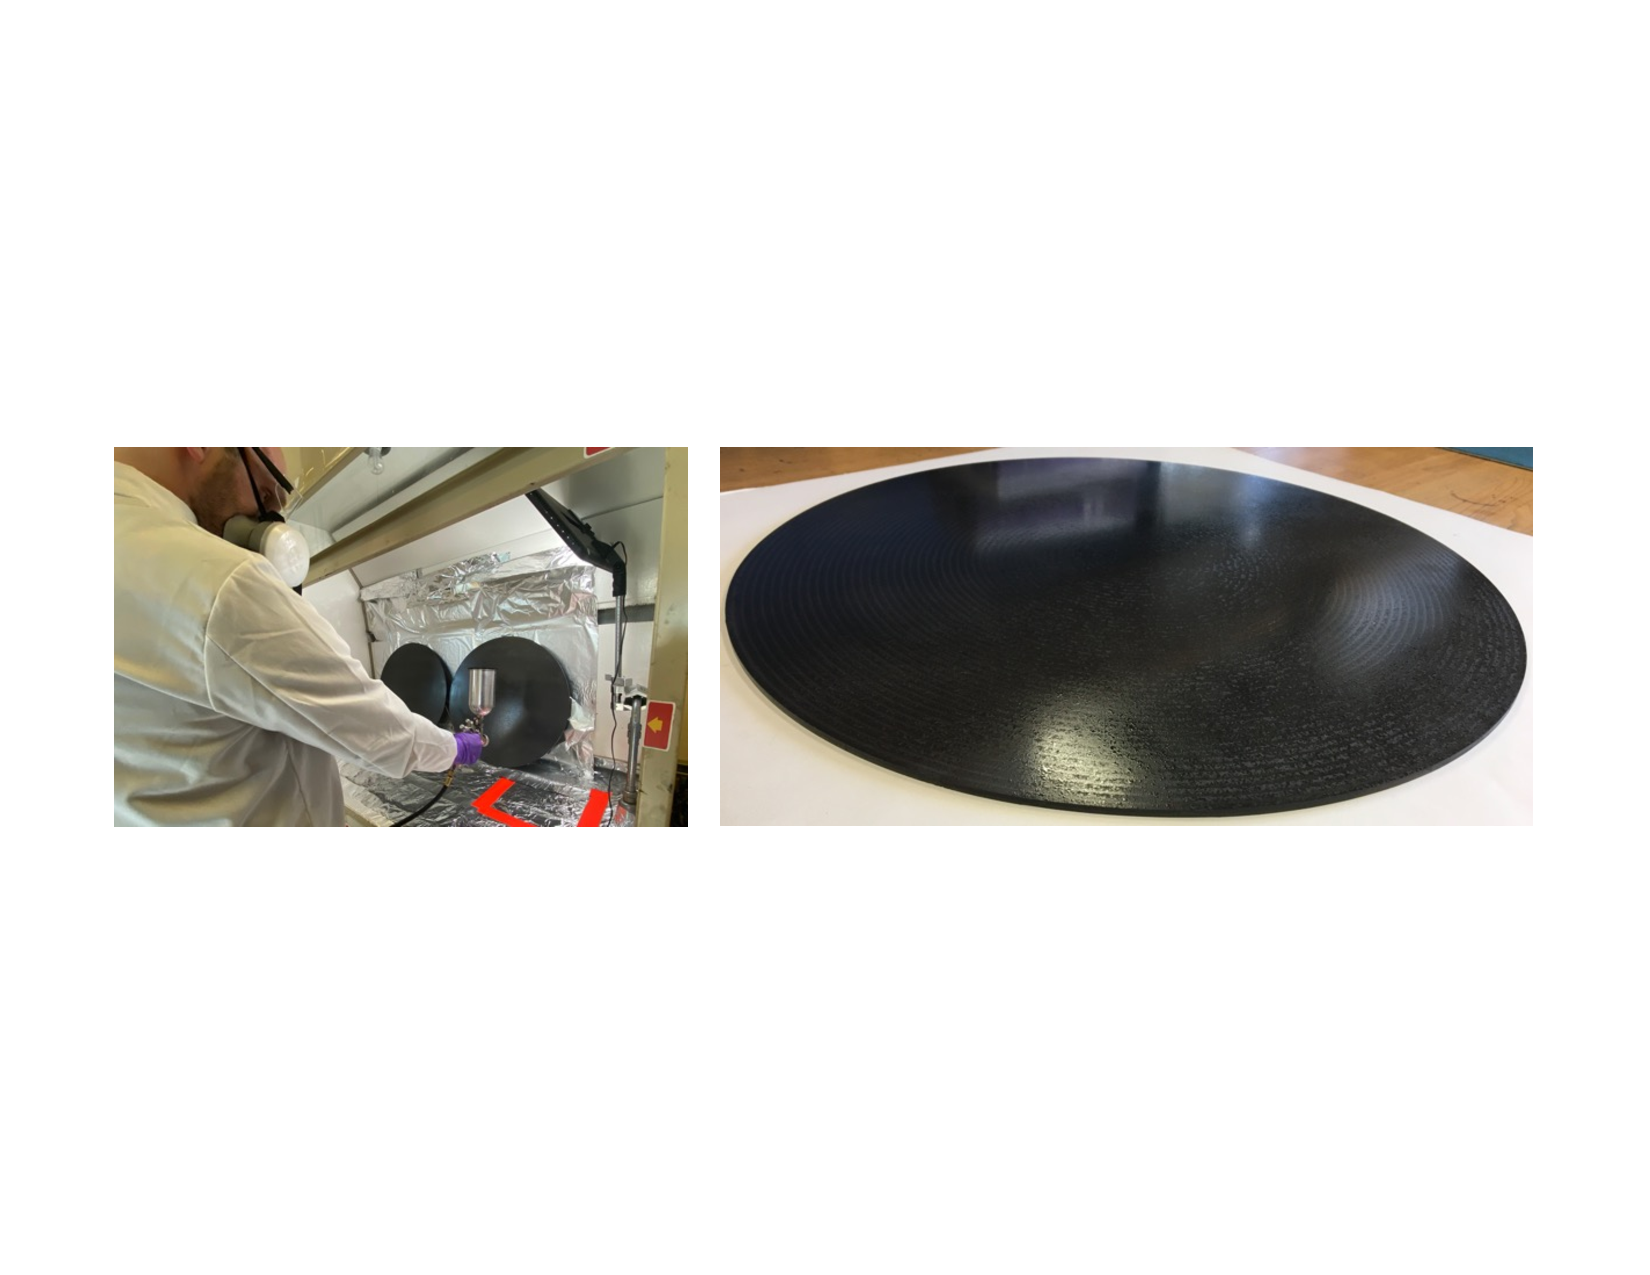
\includegraphics[width=\linewidth, trim=2cm 7cm 2cm 7cm, clip]{ARCoating/Figures/epotek_application.pdf}
    \caption[EpoTek 301-2 application for bonding Duroid 5880LZ top AR layer to the machined Stycast 2850FT bottom AR layer.]{EpoTek 301-2 application for bonding Duroid 5880LZ top AR layer to the machined Stycast 2850FT bottom AR layer. The photo on the left shows the author spraying the transparent 301-2 onto the 2850FT layer in a fume hood. The photo on the right shows the EpoTek-covered 2850FT layer after spraying has completed and before the Duroid 5880LZ is applied.}
    \label{fig:epotek_application}
\end{figure}

Figure~\ref{fig:epotek_application} shows the EpoTek 301-2 application process. When spraying, articular attention is paid to the discharge rate, the air pressure, the raster scanning speed, and the nozzle-to-surface distance. After the 301-2 coverage is deemed to be sufficient, the Duroid is laid onto the glue-covered 2850FT layer, and the assembly is vacuum bagged for the full 48-hour cure time. Utilizing atmospheric pressure to press the Duroid and Stycast-covered sapphire together ensures a large amount of pressure that is even and consistently applied.

%%%%%%%%%%%%%%%%%%%%%%%%%%%%%%%%

\subsubsection{5880LZ machining}
\label{sec:sapphire_ar_coating_epoxy_plastic_fabrication_5880LZ_machining}

Once the EpoTek 301-2 is glued down, we need to machine it to its target thickness. The standard Duroid thickness is 0.020," and the target thickness is 0.017", and therefore the machining process only needs to ``shave'' a few thousandths of an inch from the 5880LZ. In order to shear material from the Duroid sheet effectively, we use a fly cutter with a tip angled $15^{\circ}$ to the surface and running at 5,000 RPM. In a similar way to when machining the epoxy layers, we do a pre-finish cut 0.001"$\sim$0.002" above the target thickness to calibrate the $z$-offset of the spindle before proceeding to the finish cut. Because the Duroid is soft, we use a combination of gauge blocks, which act as precise spacer plates, and the Renishaw contact probe to check the layer's thickness.

%%%%%%%%%%%%%%%%%%%%%%%%%%%%%%%%

\subsubsection{Strain relieving}
\label{sec:sapphire_ar_coating_epoxy_plastic_fabrication_5880LZ_strain_relieving}

One hypothesis for the delamination of the 1~cm~$\times$~1~cm AR islands is that the laser cutting itself is seeding separation between the bottom Stycast 2850FT layer and the sapphire substrate. Therefore, during the epoxy + plastic development, we worked to better understand the impact of laser ablation on adhesion. As described in Section~\ref{sec:sapphire_ar_coating_epoxy_fabrication_strain_relief}, we use a 355~nm laser at Laserod with $\sim$~10~W to cut the strain relief lines. To improve the dicing process, we studied three parameters: the laser's pulse duration, the pulse repetition rate, and the number of passes on each cut.

The first parameter investigation is the pulse duration. It is generally known in laser machining that a shorter pulse offers better control of the heat-affected zone (HAZ)---or the area around the focus which is ``heated'' by the laser--- which leads to a cleaner cut. The HAZ is particularly important for AR strain relieving, as a large HAZ can melt the epoxy instead of ablate it, which can in turn weaken the bond between the epoxy and sapphire at the dicing lines. Because we are using a two-layer AR coating, this weakened edge can seed the top layer peeling the bottom layer away from the substrate. The corners of the square islands are particularly vulnerable to this effect, as they are exposed to twice as much total laser power from the cuts along the orthogonal directions \textit{and} the experience a larger differential thermal contraction along the island's diagonal direction.\footnote{We also investigated ``skipping'' over existing lines when cutting along the second orthogonal direction. While we think this can be done using Laserod's equipment and expertise, it fell just outside the scope of this research.} Therefore, we move from a nanosecond pulse duration to a femtosecond pulse duration, and the difference in the resulting cuts are shown by . As is evident from the scanning electron microscope images in Figure~blah, the shorter pulse duration results in a much cleaner cut with less epoxy melting.

\begin{figure}[!t]
    \centering
    \includegraphics[width=\linewidth, trim=1cm 7cm 1cm 7cm, clip]{ARCoating/Figures/laser_dicing_photos.pdf}
    \caption[Microscope photos of the laser dicing lines showing the impact of decreasing pulse duration and the number of passes.]{Microscope photos of the laser dicing lines showing the impact of decreasing pulse duration and the number of passes. The left panel shows scanning electron microscope images that compare a cut using a nanosecond pulse with that using a femtosecond pulse. The right panel shows optical microscope images through the fully-transparent backside (similar to those in Figure~\ref{fig:epoxy_delamination:b}) of one 95~mm diameter, AR-coated sapphire sample with 100\% of the passes needed to fully separate the epoxy AR islands compared to one with 150\%.}
    \label{fig:sapphire_ar_laser_dicing}
\end{figure}

The second parameter is the number of passes for each dicing line. It was found in PB-2a that if the Stycast 2850FT + 1090 AR coating was not diced all the way through to the substrate such that the epoxy islands are completely independent, the AR coating would delaminate in sheets upon cooling to cryogenic temperatures. Therefore, during the early stages of the PB-2b AR development, we would measure the number of passes needed to ``sever'' the AR coating witness sample,\footnote{The witness sample was usually a free-standing epoxy square that had delaminated from an earlier optic.} and then we would do 150\%\footnote{While 50\% extra cuts might seem like overkill, the depth of cut is not linear with the number of passes. The majority of AR coating material is ablated during the first few passes, but as the cut goes deeper, the deepening groove acts as an aperture that decreases laser power at the ablation surface. Therefore, it takes many additional passes to ensure the very bottom of the groove has undoubtedly been finished.} the measured number of passes on the optic to ensure, beyond a doubt, that the diced islands were truly independent of one another. However, as the CHWP AR development progressed, we became concerned about the effect of overcutting on the sapphire substrate. Figure~blah shows the a comparison of a sapphire sample with 100\% of the needed passes compared to one with 150\%. As is clearly seen, the overcutting cracks the sapphire substrate, and these weaknesses act similarly to melted epoxy at the edges of the squares, creating a weak point for the squares to more easily separate from the substrate. Because the PB-2b sapphire is semi-transparent, and because we only coat one side, we calibrated the number of passes by doing a test line right at the coating's edge and looking with our eyes for the laser light to shine through the bottom of the coating into the sapphire.\footnote{Even though 355~nm is technically outside of the visible spectrum, our eyes have a logarithmic rolloff into the UV, and because the UV laser is so bright, the naked eye can detect a faint blue hue when the laser is scattered.} In this way, we are able to avoid sapphire cracking at the laser edges that may seed delamination.

The third parameter is the pulse repetition rate, which when holding the raster scan speed constant determines the pulse overlap. In PB-2a, the laser was run at 100~kHz, which given a 400~mm/s raster speed an a $\sim$~30~$\mathrm{\mu m}$ laser spot size at focus corresponds to a $\sim$75\% pulse overlap. This level of overlap between adjacent pulses is often desired in laser machining to ensure a that the cut has an even edge. However, because the epoxy dicing requires $\sim$tens of passes and because we are concerned about laser-induced heating melting the epoxy and hence compromising the integrity of the adhesion, such an overlap is undesirable for the sapphire AR application, and for this reason, we reduce the repetition rate to 25~kHz.\footnote{Conservation energy suggests that decreasing the repetition rate by 4$\times$ should mandate more 4$\times$ more passes to achieve the same depth of cut. However, this relationship was found to be much less severe in practice, with the decreased rep rate only requiring a moderate increase in overall machining time.}

These three laser dicing modifications together improved the integrity of the strain relief cuts and therefore led to improved adhesion performance on 95~mm sample tests.

%%%%%%%%%%%%%%%%%%%%%%%%%%%%%%%%

\subsubsection{AR annealing}
\label{sec:sapphire_ar_coating_epoxy_plastic_fabrication_5880LZ_annealing}

The final step before thermal cycling the epoxy + plastic AR coating is to relax the Stycast 2850FT layer. During the epoxy curing process, epoxide molecules in the resin are joined by amine molecules in the catalyst to form a three-dimensional, cross-linked web of long polymer chains which form the basis of epoxy's mechanical properties. However, as the epoxy mixture phase transitions from a liquid to a solid during its cure, it shrinks, and because the cross-linking is a stochastic process, complex stress profiles develop within the epoxy's bulk. Such effects are typically not a concern when using epoxy as a standard adhesive, but because the PB-2b epoxy mixture has a large volume ($\sim$700~g of resin) and because the AR layer has a high aspect ratio (20" in diameter but only 0.010" in thickness), these stresses can compound the CTE-induced stresses during cooldown to increase the probability of delamination.

\begin{figure}[!t]
    \centering
    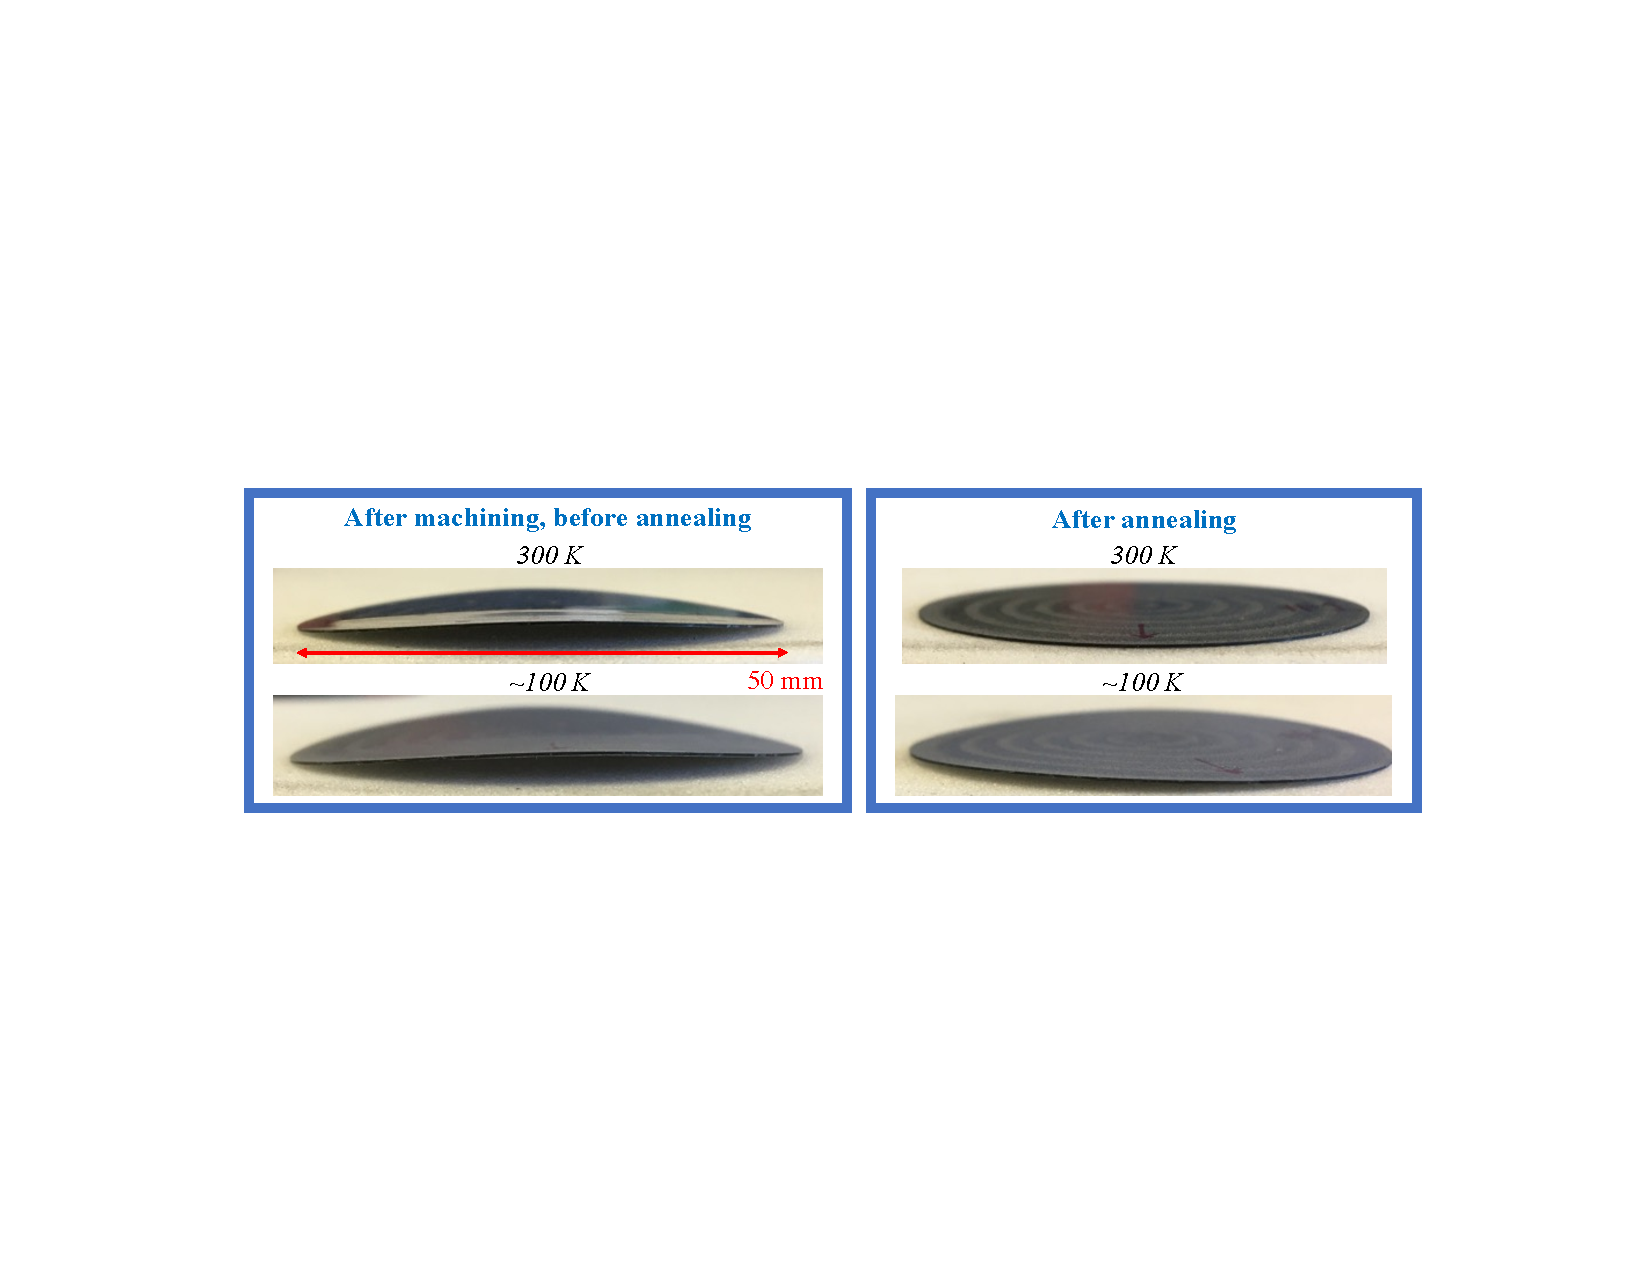
\includegraphics[width=\linewidth, trim=4cm 7.5cm 3.8cm 8cm, clip]{ARCoating/Figures/epoxy_annealing.pdf}
    \caption[Demonstration of the impact of annealing on cure-induced epoxy stress.]{Demonstration of the impact of annealing on cure-induced epoxy stress. The left panel shows a 2"-diameter, 0.010" thick epoxy sample machined to thickness in a similar manner as on the full-scale piece at both 300~K and and at $\sim$~100~K after dunking in liquid nitrogen. The piece's warping demonstrates the presence of cure-induced and machining-induced stresses. The right panel shows the same piece after annealing.}
    \label{fig:epoxy_annealing}
\end{figure}

To demonstrate the phenomenology of cure-induced stress, Figure~\ref{fig:epoxy_annealing} shows the impact of annealing on a 2"-diameter, 0.010"-thick, freestanding epoxy sample machined to thickness in the mill on a vacuum chuck in a similar way to full-sized epoxy layer as cured on the sapphire. Before any annealing, the epoxy wafer is demonstrably warped, indicating a substantial amount of cure-induced and machining-induced\footnote{While without a large sample size, we notice that all samples similar to that shown in Figure~\ref{fig:epoxy_annealing} are bowed \textit{toward} the mill bit, suggesting empirically that some stress is indeed introduced by machining. However, the fluctuations in the amount of bowing was a much large effect, also suggesting that the stochastic stresses induced during curing is the larger effect.} stresses. Guided by the advice of epoxy consultants at Ellsworth and Cumming, we alleviate these stresses via annealing.

The goal of the annealing process is to relax the epoxy while not thermally shocking it, which would do more harm and than good. We use a large Despatch oven in the main LBNL machine shop which has an in-chamber thermocouple and can house many full-scale optics simultaneously. The procedure is run automatically and includes the following steps
\begin{enumerate}
    \item Warm to $60^{\circ}$~C over 3~hours.
    \item Soak at $60^{\circ}$~C for 3~hours.
    \item Cool to $40^{\circ}$~C over 1~hour.
    \item Warm to $65^{\circ}$~C over 2 hours.
    \item Cool to $25^{\circ}$~C over 2 hours.
\end{enumerate}
When cured at room temperature, the glass transition temperature of the Stycast 2850FT is $40 \sim 60^{\circ}$~C, and therefore steps 1 and 2 are designed to soften the epoxy, allowing it to relax. After the piece is soaked at $60^{\circ}$~C, its glass transition temperature is then $60^{\circ}$, and therefore steps 2-5 are designed to once again relax the epoxy by slowly warming it to soften\footnote{Raising the epoxy above its glass transition temperature makes it slightly malleable and rubbery, but it does not reflow, and therefore the annealing process has no impact on the bond between the 2850FT and the sapphire.} and slowly cooling it to harden. This annealing profile is similar to those used for other plastics, such as polyethylenes, and therefore is a well established practice in industrial applications.

%%%%%%%%%%%%%%%%%%%%%%%%%%%%%%%%
%%%%%%%%%%%%%%%%%%%%%%%%%%%%%%%%

\subsection{Duroid performance}
\label{sec:sapphire_ar_coating_epoxy_plastic_duroid_performance}

In a similar way to with the epoxy-only AR coating, we consider both the cryo-mechanical and optical performance of the Stycast 2850FT + Duroid 5880LZ coating in this section. Given our experiences with the epoxy coating, we focused the majority of our R\&D efforts on the quality of the cryogenic adhesion, knowing that if the coating is survives thermal cycling, its optical performance will likely be well-described by a simulation using measured optical constants and thicknesses for the individual layers. 

%%%%%%%%%%%%%%%%%%%%%%%%%%%%%%%%

\subsubsection{Optical performance}
\label{sec:sapphire_ar_coating_epoxy_plastic_duroid_optical_performance}

The first sample that we fabricated for optical testing was a 6"-diameter, 1/8"-thick piece of alumina coated on both sides and is shown in Figure~\ref{fig:epoxy_duroid_alumina_warm:a}. This piece was first measured at ambient temperature using two separate coherent-source setups: one that measures reflectivity (University of Michigan) and one that measures transmissivity (UC Berkeley). Both setups have tunable sources that generate narrow-band signals which are stepped in frequency, and a coherent detector is used to measure both amplitude and phase of the reflected/transmitted signal through the sample. The results of the measurement are shown in Figure~\ref{fig:epoxy_duroid_alumina_warm:b}, and the measured reflectivity at (90, 150)~GHz is (0.6, 1.1)\%. The substantial loss seen in the transmissivity measurement is due to the large loss tangents of both the Stycast 2850FT and the Duroid 5880LZ at room temperature. However, measurements of each AR material at 100~K show substantial reductions in their loss tangents at cryogenic temperatures, and combination of those individual-layer measurements and the ambient measurements in Figure~\ref{fig:epoxy_duroid_alumina_warm:b} suggest $\approx$~98\% transmission in both bands at the CHWP's operating temperature.\footnote{While this statement is made specifically for the SO bands, it also applies to PB-2b, which observes at nearly identical frequencies.}

\begin{figure}[!t]
    \centering
    \subfloat[\label{fig:epoxy_duroid_alumina_warm:a}]{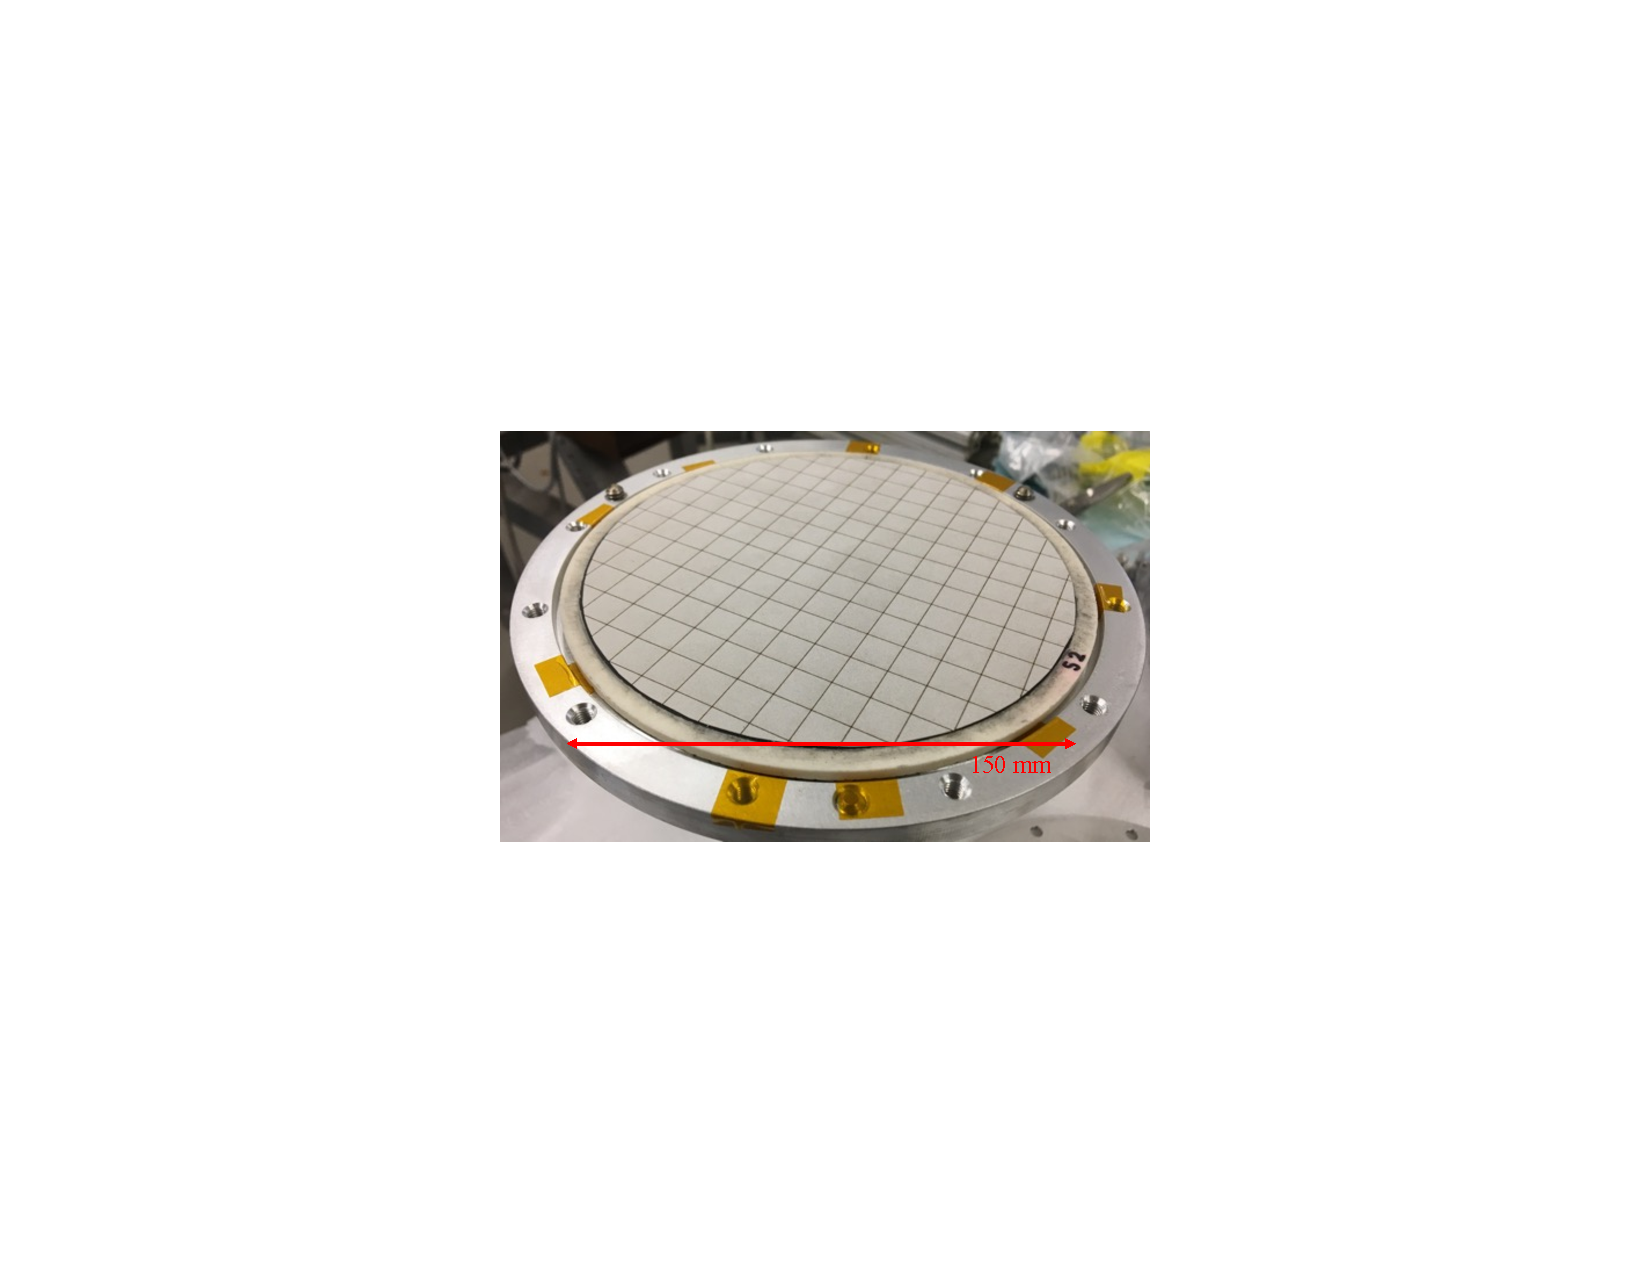
\includegraphics[width=0.5\linewidth, trim=8cm 7cm 8cm 7cm, clip]{ARCoating/Figures/epoxy_duroid_on_alumina_warm.pdf}}
    \hfill
    \subfloat[\label{fig:epoxy_duroid_alumina_warm:b}]{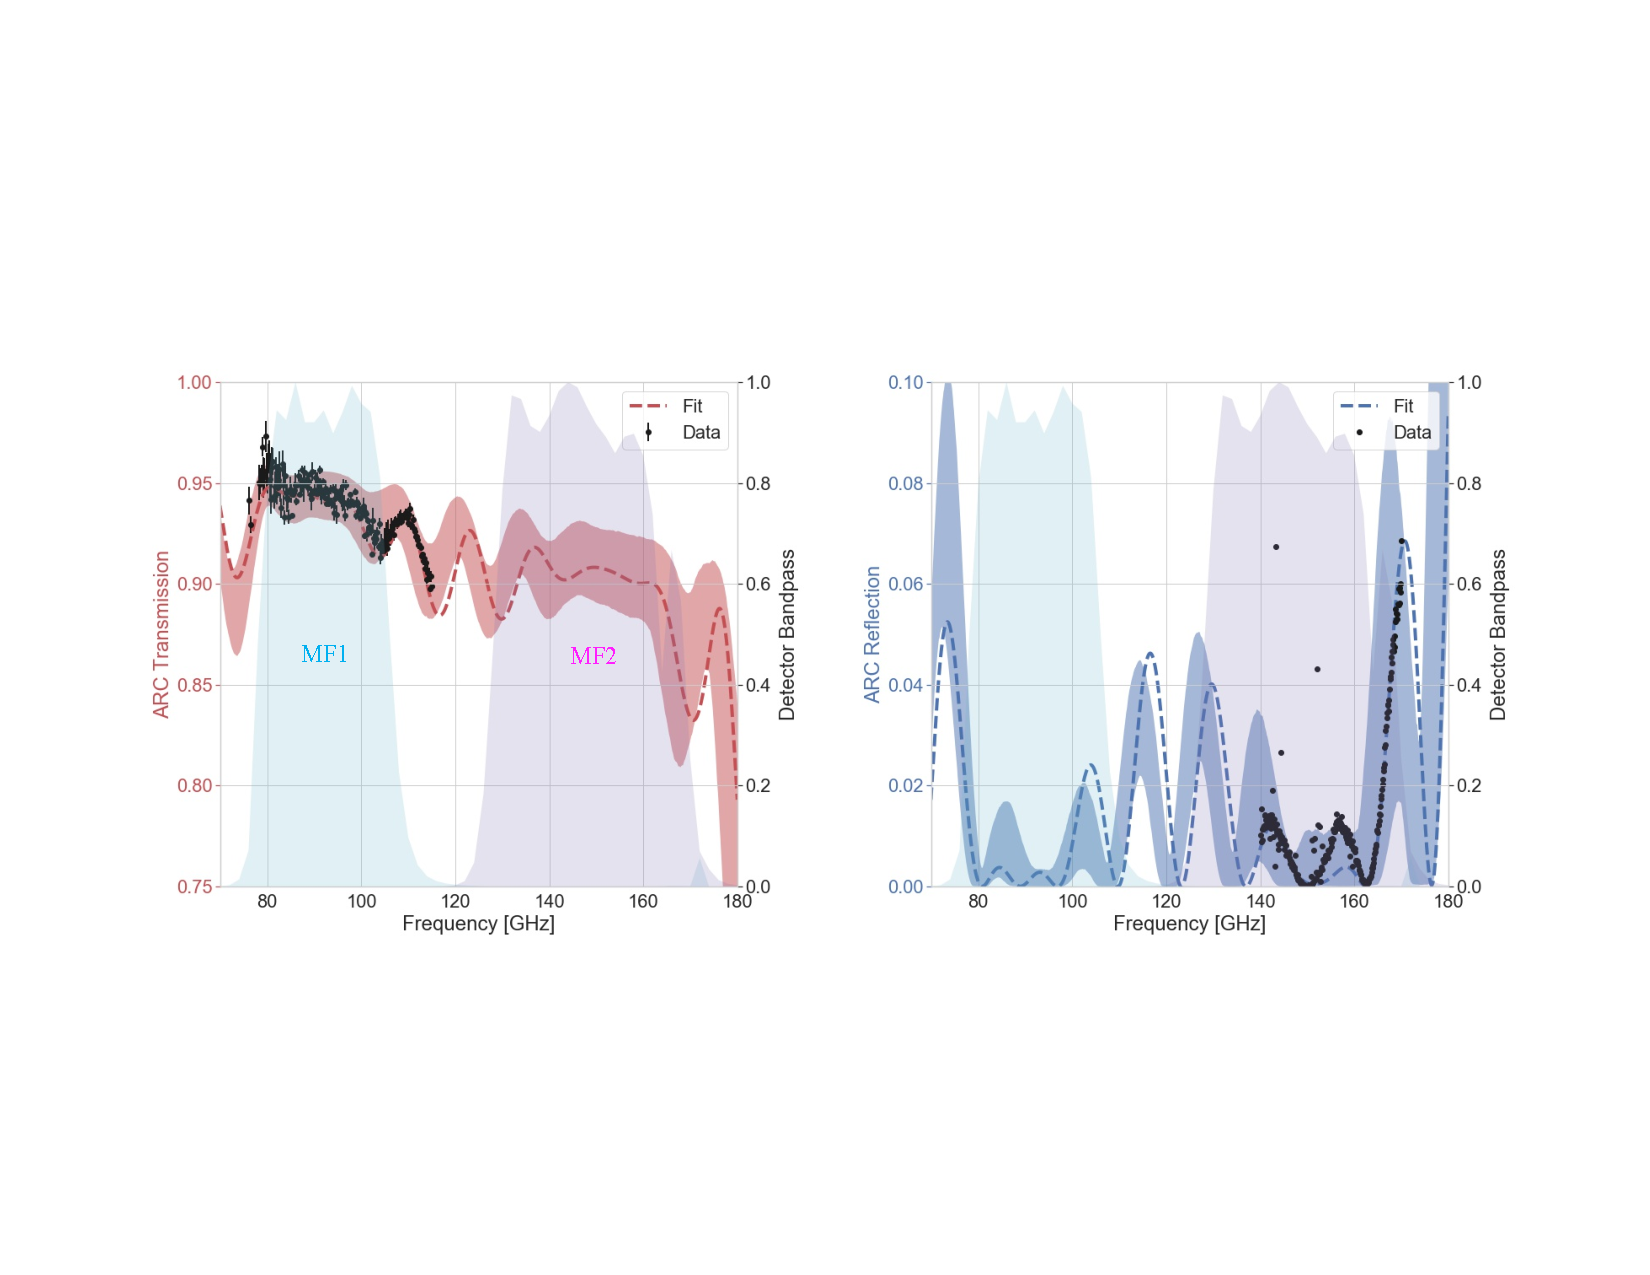
\includegraphics[width=\linewidth, trim=2cm 5.5cm 2cm 6cm, clip]{ARCoating/Figures/epoxy_duroid_on_alumina_warm_measurement.pdf}}
    \caption[A warm measurement of epoxy + Duroid on a 6" alumina sample.]{A warm measurement of epoxy + Duroid on a 6" alumina sample. Figure~\ref{fig:epoxy_duroid_alumina_warm:a} shows a photo of the sample at room temperature before any thermal cycles. The sample is coated on both sides, and the dicing pattern is 1~cm~$\times$~1~cm, just as was done for the epoxy-only coatings. Figure~\ref{fig:epoxy_duroid_alumina_warm:b} shows the results of the transmissivity (left) and reflectivity (right) measurements. The dotted lines are fits to the black data points, and the shaded bands are the expectation based on measurements of the individual-layer indexes, loss tangents, and thicknesses. The agreement is largely consistent, and the observed frequency shift between the fit and prediction is likely due to systematic effects in the measurement of the underlying alumina substrate, which was performed independently and is not shown. The cyan and magenta shaded regions are the Simons Observatory 90 and 150~GHz detector bands.}
    \label{fig:epoxy_duroid_alumina_warm}
\end{figure}

Motivated by both the outstanding reflectivity of the warm sample in Figure~\ref{fig:epoxy_duroid_alumina_warm} and by the stability of each AR coating's materials property down to cryogenic temperatures, we then measure the sample's reflectivity at $\approx$~140~K with the same reflectivity setup used for the warm measurement except with the sample connected to a bath of liquid nitrogen. Careful and thorough analysis was done to understand the impact of adding LN2---which has a refractive index of $n_{\mathrm{LN2}} \approx 1.2$ at mm wavelengths---to the optical path, and system of heaters was used to prevent ice from forming on the Styrofoam\footnote{Styrofoam, which is expanded polystyrene, is essentially transparent at $\sim$~100~GHz.} bucket that contained the cryogen. In addition, several calibration measurements were made with both a fully-reflective plate and a slab of high-density polyethylene (HDPE) to cross check for systematic effects that may have been introduced by adding the cryogen infrastructure. The results of the measurement are shown in Figure~\ref{fig:epoxy_duroid_alumina_cold}.

\begin{figure}[!t]
    \centering
    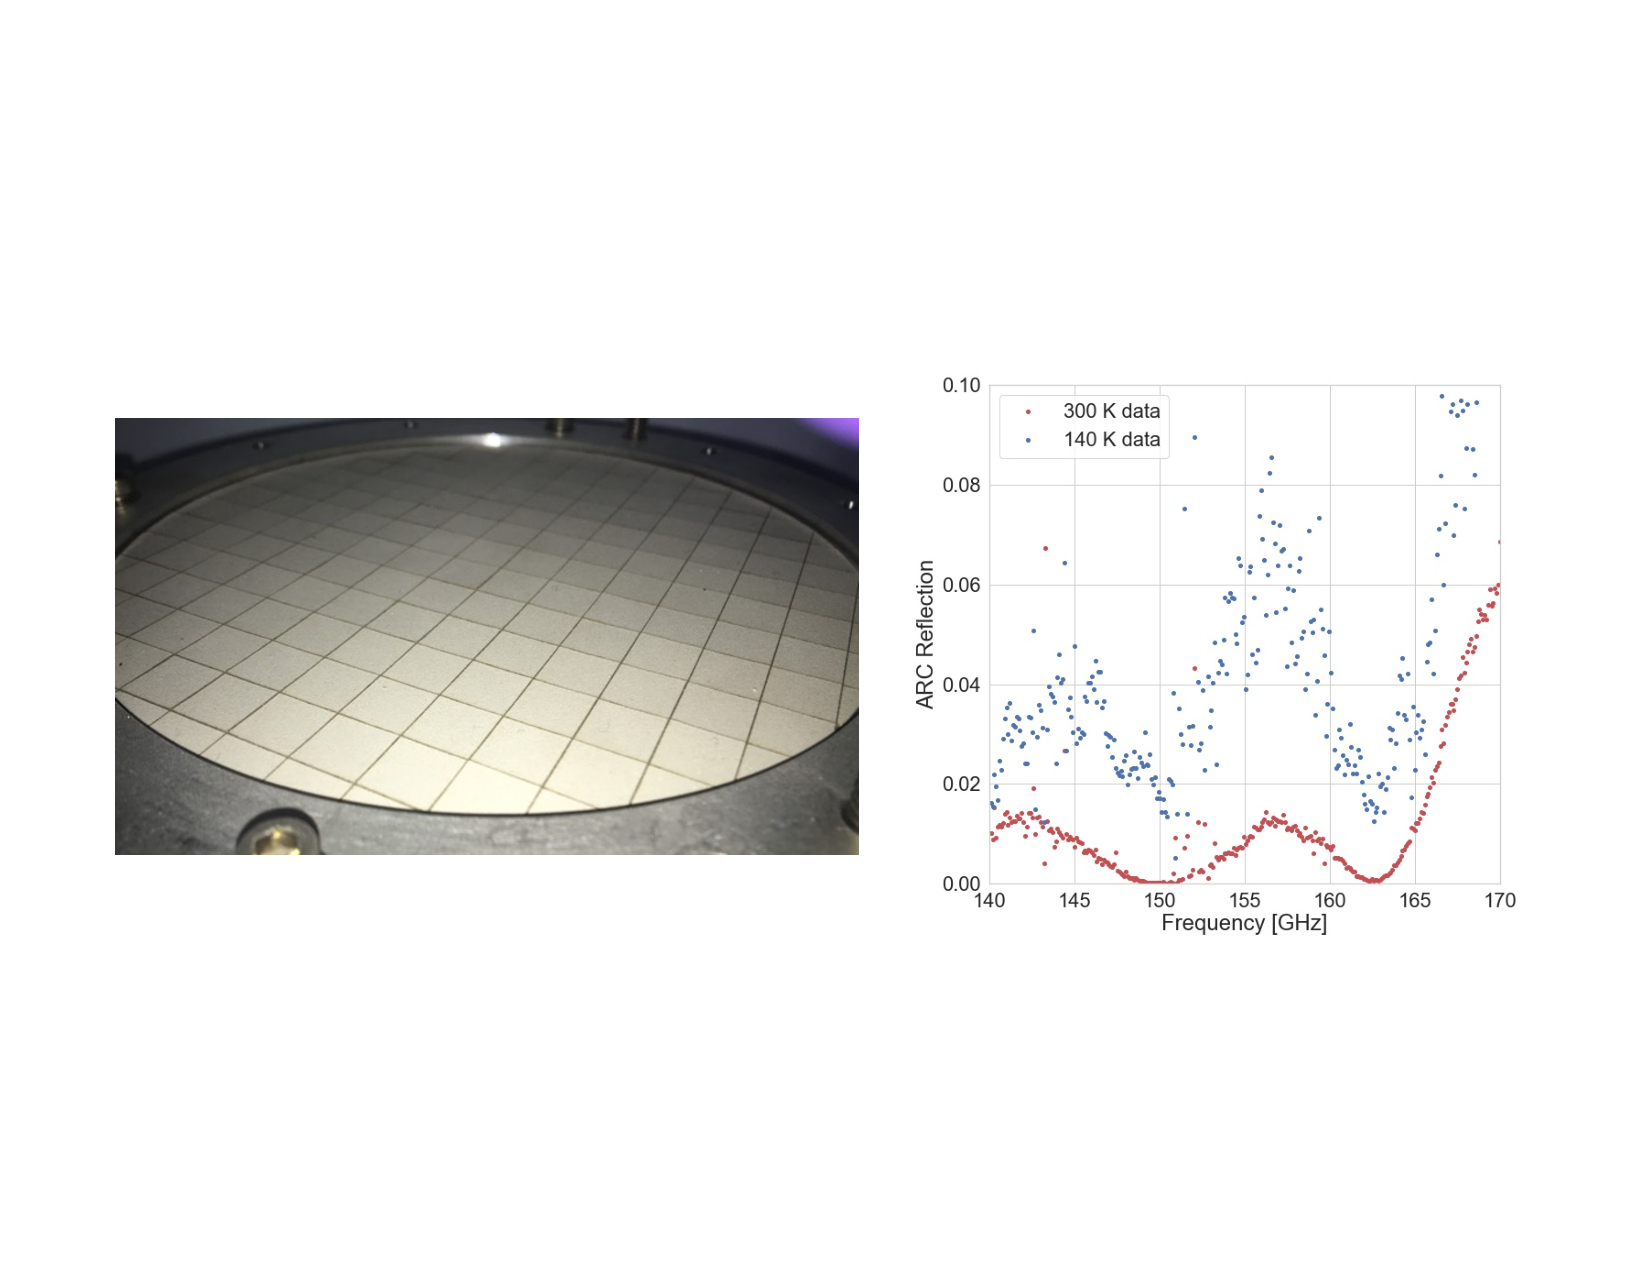
\includegraphics[width=\linewidth, trim=2cm 5.5cm 2cm 5.5cm, clip]{ARCoating/Figures/epoxy_duroid_on_alumina_cold.pdf}
    \caption[A cryogenic measurement of epoxy + Duroid on a 6" alumina sample.]{A cryogenic measurement of epoxy + Duroid on a 6" alumina sample. The right panel shows that the square islands are peeling at the dicing lines when the sample is cooled to $\sim$140~K, and the right panel shows that the reflectivity increases between 300~K and 140~K as a result.}
    \label{fig:epoxy_duroid_alumina_cold}
\end{figure}

Unfortunately, a similar effect to that seen with the epoxy-only AR coating is also seen with the epoxy + Duroid. Upon cooling, the epoxy squares delaminate at the dicing lines, and the independent islands curl to form an air gap between the bottom 2850FT AR layer and the alumina substrate. While the resulting increase in reflection is not as severe with the Duroid (compare Figure~\ref{fig:epoxy_delamination} to Figure~\ref{fig:epoxy_duroid_alumina_cold}), the resulting loss in efficiency is 3$\sim$4$\times$ larger than nominal, necessitating either another change in AR technology or a campaign to improve adhesion.

%%%%%%%%%%%%%%%%%%%%%%%%%%%%%%%%

\subsubsection{Cryo-mechanical performance}
\label{sec:sapphire_ar_coating_epoxy_plastic_duroid_cryo_mechanical_performance}

While the optical evaluation of the epoxy + Duroid coating described in the previous subsection indicates that partial delamination at cryogenic temperatures leads to increased reflectivity, the impressiveness of the \textit{warm} measurement spurred an additional R\&D campaign to ``fix'' the AR coating by improving cryogenic adhesion. This R\&D was largely performed on 95~mm-diameter sapphire samples, which were quick to coat, cheap to laser dice, and easy to cool, all of which enabled quick-turnaround experimentation. A $\sim$dozen such iterations in tandem with auxiliary research led to many of the fabrication advancements presented in Section~\ref{sec:sapphire_ar_coating_epoxy_plastic_fabrication}, and many of these process improvements indeed improved coating robustness on these small samples. Because the length scale of differential-CTE-induced stress is set by the 1~cm pitch of the strain relief cuts, the belief was that these improvements on small pieces would scale to the 20"-diameter sapphire. Therefore, once the epoxy + Duroid fabrication process was demonstrated on the small pieces, we moved to coat the PB-2b CHWP, which involves coating one side of the two outermost sapphire pieces in the Pancharatnam stack (see Section~\ref{sec:ahwp_performance} for more details about the achromatic half-wave plates).

\begin{figure}[!t]
    \centering
    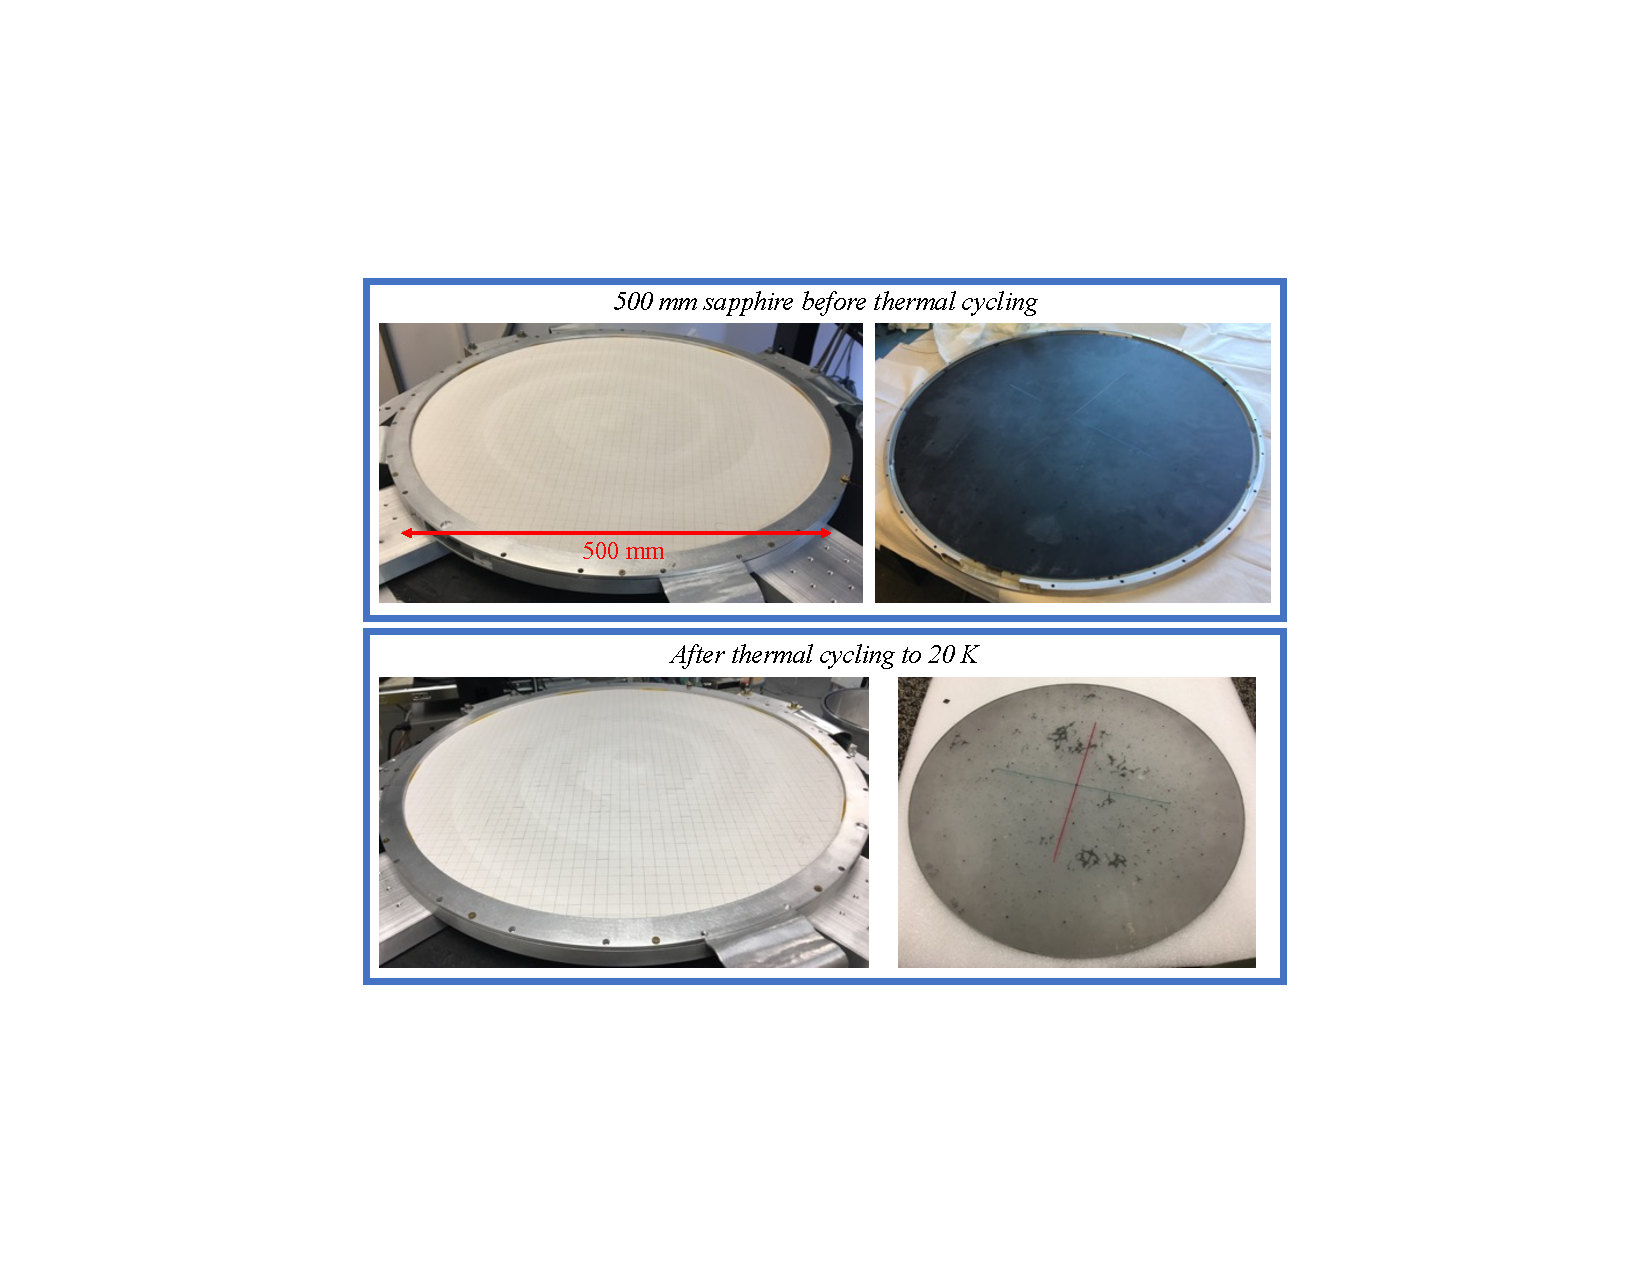
\includegraphics[width=0.8\linewidth, trim=6cm 4.5cm 6cm 4.5cm, clip]{ARCoating/Figures/epoxy_duroid_sapphire_thermal_cycle.pdf}
    \caption[The results of thermal cycling epoxy + Duroid on 20"-diameter sapphire to cryogenic temperatures.]{The results of thermal cycling epoxy + Duroid on 20"-diameter sapphire to cryogenic temperatures. The top panel shows one of the PB-2b windows before cooling, and the bottom panel shows the same piece after cooling. The contrast in the color observed through the sapphire's semi-transparent backside, as shown in the right photos, shows that the delamination is both widespread and more substantial than witnessed on 95~mm test samples.}
    \label{fig:epoxy_duroid_full_scale_thermal_cycle}
\end{figure}

The results of thermal cycling the PB-2b sapphire to $\approx$~20~K in a vacuum chamber over the course of $\approx$~2~days is shown in Figure~\ref{fig:epoxy_duroid_full_scale_thermal_cycle}. As is most clearly seen in the photos through the sapphire's semi-transparent backside, the AR coating delaminated over $>$~90\% of the surface, a result that was much worse than anticipated from cryogenic cycles of 95~mm pieces fabricated using an $sim$identical process.

%%%%%%%%%%%%%%%%%%%%%%%%%%%%%%%%
%%%%%%%%%%%%%%%%%%%%%%%%%%%%%%%%

\subsection{Duroid assessment}
\label{sec:sapphire_ar_coating_epoxy_plastic_duroid_assessment}

Despite its excellent performance at 300~K and its stable material properties down to cryogenic temperatures, the epoxy + Duroid coating does not solve the problems of delamination seen with the already defunct epoxy-only technology. Therefore, sapphire pieces shown in Figure~\ref{fig:epoxy_duroid_full_scale_thermal_cycle} were deemed unfit for deployment on PB-2b. The degree of cryogenic delamination witnessed on the 20" pieces was surprising. As mentioned in Section~\ref{sec:sapphire_ar_coating_epoxy_plastic_duroid_cryo_mechanical_performance}, the philosophy behind developing the epoxy + Duroid AR process on 95~mm-diameter sapphire was that the length scale of differential-CTE-induced stress is the 1~cm pitch of the laser cuts, and therefore a robust demonstration on small pieces should scale reasonably well to a large pieces. However, this philosophy proved to be flawed, and in this section we pose several theories that are being considered in ongoing AR coating R\&D.

The first theory behind the epoxy + Duroid's full-scale delamination is that the adhesion degrades with diameter. During its cure, Stycast 2850FT  shrinks by 0.3\% due to the formation of tight-knit cross-linked polymer chains that give the adhesive its mechanical strength. This shrinkage occurs slowly during the cure\footnote{According to conversations with consultants at Ellsworth Adhesives, the shrinkage is not linear in time, but instead the vast majority of the cross linking occurs during the first $\sim$~6~hours of the cure.} and amounts to a $\Delta L =$~(25, 150)~$\mathrm{\mu m}$ for the (95, 500)~mm diameter samples. Because the coating is strain relieved before cooling, this stress should be relieved before the coating is stressed. However, it may be that epoxy's shrinking \textit{while} curing degrades its adhesion to the sapphire or even weakens the sapphire itself, infesting the surface with microfractures. Then, when the part is cooled, the weakened bondline cannot withstand the additional stress. This effect would be more impactful the larger the piece and therefore could explain the discrepant performance between 500~mm and 95~mm pieces. The second theory is that the sapphire itself may make a difference. While there is no evidence to suggest that large sapphire pieces would be more vulnerable than small pieces to damage during the AR fabrication process, this is a possibility that warrants some investigation and monitoring as AR development continues. The final theory is that the base temperature of the thermal cycle makes a difference, and that the 500~mm piece failed because we cooled it to 20~K and the 95~mm pieces did not because we cooled them to 80~K. Most materials---including sapphire and plastics---undergo the vast majority of thermal contraction upon cooling above $\sim$~100~K, and therefore cryo-mechanical tests to LN2 temperatures are typically indicative of mechanical robustness to lower temperatures. However, it could be that an unexpected physical mechanism between 80~K and 20~K causes the coating to fail between those two temperatures. This hypothesis can be tested by making small samples and cooling them to 20~K.

In summary, replacing the top Stycast 1090 layer in the epoxy-only AR coating with Duroid 5880LZ in the epoxy + plastic AR coating improves ambient optical performance and \textit{should} improve cryo-mechanical robustness due to Duroid having a lower CTE and tensile modulus than Stycast; however, we instead see widespread adhesive failure on full-scale sapphire pieces that requires further R\&D to validate this technology for use on the PB-2b CHWP.

%%%%%%%%%%%%%%%%%%%%%%%%%%%%%%%%
%%%%%%%%%%%%%%%%%%%%%%%%%%%%%%%%
%%%%%%%%%%%%%%%%%%%%%%%%%%%%%%%%

\section{Ongoing work}
\label{sec:sapphire_ar_coating_ongoing_work}

At the time of this dissertation, the PB-2b CHWP remains without an AR coating. The task of AR coating the sapphire is the final outstanding item for the PB-2b CHWP, and there are several research areas that are being pursued in parallel. We cover each of them briefly in this section, highlighting the strengths and challenges of each technology.

%%%%%%%%%%%%%%%%%%%%%%%%%%%%%%%%
%%%%%%%%%%%%%%%%%%%%%%%%%%%%%%%%

\subsection{Epoxy + Duroid}
\label{sec:sapphire_ar_coating_ongoin_work_epoxy_duroid}

The primary problem with the Stycast 2850FT + Duroid 5880LZ coating is the adhesion between the bottom layer and the sapphire. One of the hypotheses for the poor adhesion is that Stycast shrinkage when curing on the sapphire's surface prevents a sufficiently robust bond. To solve this problem, we aim to cure the epoxy \textit{off of} the sapphire as a standalone wafer, glue this cured wafer to the sapphire using a thin layer of EpoTek 301-2, machine the glued wafer wafer to the target thickness, and proceed with the rest of the procedure as presented in Sections~\ref{sec:sapphire_ar_coating_epoxy_fabrication} and~\ref{sec:sapphire_ar_coating_epoxy_plastic_fabrication}. The primary challenge with this technique is to achieve an EpoTek layer that is sufficiently thin with respect to the wavelength and is free of air bubbles. The Stycast wafer technique is currently being cryo-mechanically demonstrated on both small and large samples, and an optical measurement is set to follow soon after.

%%%%%%%%%%%%%%%%%%%%%%%%%%%%%%%%
%%%%%%%%%%%%%%%%%%%%%%%%%%%%%%%%

\subsection{Mullite + Duroid}
\label{sec:sapphire_ar_coating_mullite_duroid}

The problematic layer in the Stycast 2850FT + Duroid 5880LZ AR coating is the bottom Stycast 2850FT. Therefore, one strategy is to replace that layer with a material that will better adhere to the sapphire. PB-2a used two different coatings on its alumina optics: epoxy-only on the curved surfaces of the reimaging lenses (see Section~\ref{sec:sapphire_ar_coating_epoxy} for details) and mullite + Skybond~\cite{Inoue2016} on the flat surfaces. Mullite is a silicate with chemical composition $\mathrm{3Al_{2}O_{3}2SiO_{2}}$, has a refractive index of $n_{\mathrm{mullite}} = 2.52$, and most importantly has a small coefficient of thermal expansion that is well matched to that of sapphire. Skybond is an expanded polyimide foam whose density is tunable and for PB-2a has an index of $n_{\mathrm{Skybond}} = 1.43$. This coating combination worked well on PB-2a's flat surfaces, achieving reflectivities of (2.1, 1.1)\% in the (90, 150)~GHz bands. The reason the mullite-Skybond coating was not considered for the PB-2b CHWP is shortly after the PB-2a fabrication, Skybond manufacturing was discontinued. However, we nonetheless seek to leverage the success of the mullite + Skybond development by replacing the top layer with Duroid 5880LZ, which has an index of $n_{\mathrm{5880LZ}} = 1.41$ that is close to that of Skybond.

The mullite is applied via \important{thermal spraying} (sometimes called ``plasma spraing''), which involves heating a mullite powder to the point of converting it to a plasma. This mullite plasma is then accelerated using an electric field and discharge through a nozzle to create a hot mullite spray that cools and adheres to the surface upon contact. Thermal spraying is an attractive technique for mm-wave AR coatings because the spray parameters---such as deposition rate, raster scan speed, nozzle distance, etc.---can be tuned to control layer uniformity and thickness precisely. Mullite spraying is conducted at a commercial company in Japan and is facilitated by our collaborators in the KEK High Energy Research Organization and the University of Tokyo. After the mullite layer is applied, we then use EpoTek 302-1, applied using in an aerosolized form as described Section~\ref{sec:sapphire_ar_coating_epoxy_plastic_fabrication_5880LZ_application} to apply the Duroid 5880LZ layer, which is pre-machined to the target thickness. At this point, the Duroid is diced using a razor blade into $\sim$5~$\times$~5~cm square islands, and the mullite layer is left untouched. 

The mullite + Duroid coating has shown both promising optical and cryo-mechanical performance on small samples, and large-scale cryo-mechanical testing on both alumina and sapphire is ongoing. Motivated by the success of early-stage mullite testing and by the cryo-compatible versatility of EpoTek 301-2, we are also investigating a three-layer AR coating of mullite + Duroid 6002 ($n_{\mathrm{6002}} \approx 1.7$) + porous PTFE ($n_{\mathrm{pPTFE}} \approx 1.2$), which would achieve $<$~1\% reflectivity in both PB-2b bands. This technology leverages many of the lessons we have learned during the sapphire AR coating development campaign and would be an attractive application for both Simons Observatory and CMB Stage 4.

